\documentclass[10pt, letterpaper]{report}
% !TeX program = xelatex
%==================PREAMBOLO=======================%
\usepackage[utf8]{inputenc}
\usepackage{psvectorian}
\usepackage{pgfplots}
\usepackage[Rejne]{fncychap}
\usepackage[export]{adjustbox}
\usepackage[T1]{fontenc}
\usepackage{lmodern}
\usepackage{blindtext}
\usepackage{pdfpages}
\usepackage[shortlabels]{enumitem}
\usepackage{moresize}
\usepackage{graphicx} % Required for inserting images
\usepackage{hyperref}
\usepackage{listings}
\usepackage[table,xcdraw]{xcolor}
\usepackage{amssymb}
\usepackage{amsmath}
\usepackage[english]{babel}
\usepackage{nicefrac, xfrac}
\usepackage{tikz}
\usepackage{tikz-3dplot}
\usepackage{tikz-cd}
\usepackage{mathrsfs} 
\usepackage{titletoc}
\usepackage{fancyhdr}
\usepackage{psvectorian,lipsum}
\usepackage{fourier-orns}
\usepackage{lipsum}
\usepackage{wrapfig}
\usepackage{multicol}
\usepackage[paper=a4paper,left=25mm,right=25mm,bottom=25mm,top=25mm]{geometry}
\definecolor{light-gray}{gray}{0.95}
\definecolor{cop}{HTML}{f7ecd7}
\definecolor{copAut}{HTML}{ababab}
\definecolor{copAut2}{HTML}{c3c3e6}
\definecolor{purcop}{HTML}{d0d3db}
\definecolor{sapienza}{HTML}{660f1d}
\definecolor{lightSapienza}{HTML}{e3d3d5}
\definecolor{darkgreen}{HTML}{008000}
\definecolor{cartaRiciclata}{HTML}{fcfcf7}
\newcommand{\redText}[1]{\color{red}#1\color{black}}
\newcommand{\code}[1]{\colorbox{light-gray}{\texttt{#1}}}
\newcommand{\codee}[1]{\colorbox{white}{\texttt{#1}}}
\newcommand{\K}{{\mathbb K}}
\newcommand{\notimplies}{%
  \mathrel{{\ooalign{\hidewidth$\not\phantom{=}$\hidewidth\cr$\implies$}}}}
\newcommand{\flowerLine}{ \begin{center}\decofourleft\hphantom{ }\decoone\hphantom{ }\decofourright\hphantom{}\hphantom{aa}
\decofourleft\hphantom{ }\decoone\hphantom{ }\decofourright\hphantom{}\hphantom{aa}
\decofourleft\hphantom{ }\decoone\hphantom{ }\decofourright\hphantom{}\hphantom{aa}
\decofourleft\hphantom{ }\decoone\hphantom{ }\decofourright\hphantom{}\hphantom{aa} 
\decofourleft\hphantom{ }\decoone\hphantom{ }\decofourright\hphantom{}\hphantom{aa}
\decofourleft\hphantom{ }\decoone\hphantom{ }\decofourright\hphantom{}\hphantom{aa}
\decofourleft\hphantom{ }\decoone\hphantom{ }\decofourright\hphantom{}\hphantom{aa}
\decofourleft\hphantom{ }\decoone\hphantom{ }\decofourright\hphantom{}\hphantom{aa}
\decofourleft\hphantom{ }\decoone\hphantom{ }\decofourright\hphantom{}\hphantom{aa}
\end{center}}
\definecolor{g}{RGB}{60, 50, 50}
\newcommand{\textg}[1]{\color{g}{\textbf{#1}}\color{black}}
\newcommand{\teo}[1]{{\large\color{sapienza}\textbf{Teorema #1 :\hphantom{a}}}}
\newcommand{\defi}[1]{{\large\color{sapienza}\textbf{Definizione #1 :\hphantom{a}}}}
\newcommand{\claim}[1]{{\color{sapienza}\textbf{Claim #1 :\hphantom{a}}}}
\newcommand{\lemma}[1]{{\color{sapienza}\textbf{Lemma #1 :\hphantom{a}}}}
\newcommand{\dimo}[1]{{\color{sapienza}\textbf{Dimostrazione #1 :\hphantom{a}}}}
\newcommand{\prop}[1]{{\color{sapienza}\textbf{Proposizione #1 :\hphantom{a}}}}
\newcommand\greybox[1]{%
  \vskip\baselineskip%
  \par\noindent\colorbox{light-gray}{%
    \begin{minipage}{\textwidth}#1\end{minipage}%
  }%
  \vskip\baselineskip%
}
\newcommand\sapbox[1]{%
  \vskip\baselineskip%
  \par\noindent\colorbox{lightSapienza}{%
    \begin{minipage}{\textwidth}#1\end{minipage}%
  }%
  \vskip\baselineskip%
}
\newcommand{\ridFunc}{{f:\Sigma^*\rightarrow \Sigma^*}}
\newcommand{\rid}{{\le_m^P}}
\newcommand{\Z}{{\mathbb Z}}
\newcommand{\blank}{{\sqcup}}
\newcommand{\Prob}{{\mathbb P}}
\newcommand{\R}{{\mathbb R}}
\newcommand{\VA}{{\mathbb E}}
\newcommand{\N}{{\mathbb N}}
\newcommand{\quat}{{\mathbb H}}
\newcommand{\C}{{\mathbb C}}
\newcommand{\Sn}{{\mathcal S_n}}
\newcommand{\An}{{\mathcal A_n}}
\newcommand{\E}{{\mathcal E}}
\newcommand{\B}{{\mathcal B}}
\newcommand{\mcm}{{\text{mcm}}}
\newcommand{\rg}{{\text{rg}}}
\newcommand{\ve}{{\bar v}}
\newcommand{\spaz}{{\text{\hphantom{aa}}}}
\newcommand{\MCD}{{\text{MCD}}}
\newcommand{\tc}{{\text{ tale che }}}
\newcommand{\supp}{{\text{Supp}}}
\newcommand{\acc}{\\\hphantom{}\\}
\newcommand{\esempio}[1]{{\acc\large\color{sapienza}\textbf{Esempio #1 \hphantom{a}}\acc}}
\newcommand{\bra}[1]{\langle #1 \rangle}
\newcommand{\aut}{{\text{Aut}}}
\newcommand{\Span}{{\text{Span}}}
\newcommand{\End}{{\text{End}}}
\newcommand{\cen}{{\text{Centro}}}
\newcommand{\norm}{{\unlhd}}
\newcommand{\ciclS}{{\left \langle }}
\newcommand{\ciclE}{{\right \rangle }}
\newcommand{\boxedMath}[1]{\begin{tabular}{|c|}\hline \texttt{#1} \\ \hline\end{tabular} :} 
\newcommand{\shell}[1]{\colorbox{black}{\textcolor{white}{\texttt{#1}}}}
\newcommand{\eqImportante}[1]{\begin{center}\huge\lefthand\hphantom{a}
    \normalsize\texttt{#1}
    \hphantom{aaa}\huge\righthand\end{center}}

\fancyhf{}
\pagestyle{fancy}
\usepackage{pgf-pie}  
\usetikzlibrary{positioning}

\renewcommand{\headrule}{%
\vspace{-8pt}\hrulefill
\raisebox{-2.1pt}{\quad\decothreeleft\decotwo\decothreeright\quad}\hrulefill}

%sta roba serve per il codice C
\definecolor{mGreen}{rgb}{0,0.6,0}
\definecolor{mGray}{rgb}{0.5,0.5,0.5}
\definecolor{mPurple}{rgb}{0.58,0,0.82}
\definecolor{backgroundColour}{rgb}{0.95,0.95,0.92}

\lstdefinestyle{CStyle}{
    backgroundcolor=\color{backgroundColour},   
    commentstyle=\color{mGreen},
    keywordstyle=\color{magenta},
    numberstyle=\tiny\color{mGray},
    stringstyle=\color{mPurple},
    basicstyle=\footnotesize,
    breakatwhitespace=false,         
    breaklines=true,                 
    captionpos=b,                    
    keepspaces=true,                 
    numbers=left,                    
    numbersep=5pt,                  
    showspaces=false,                
    showstringspaces=false,
    showtabs=false,                  
    tabsize=2,
    language=C
}
\lstdefinestyle{CppStyle}{
    backgroundcolor=\color{backgroundColour},   
    commentstyle=\color{mGreen}\ttfamily,
    morecomment=[l][\color{magenta}]{\#}
    keywordstyle=\color{blue}\ttfamily,
    numberstyle=\tiny\color{mGray},
    stringstyle=\color{red}\ttfamily,
    basicstyle=\ttfamily,
    breakatwhitespace=false,         
    breaklines=true,                 
    captionpos=b,                    
    keepspaces=true,                 
    numbers=left,                    
    numbersep=5pt,                  
    showspaces=false,                
    showstringspaces=false,
    showtabs=false,                  
    tabsize=2,
    language=C
}
\lstset{language=C++,
                basicstyle=\ttfamily,
                keywordstyle=\color{blue}\ttfamily,
                stringstyle=\color{red}\ttfamily,
                commentstyle=\color{green}\ttfamily,
                morecomment=[l][\color{magenta}]{\#}
}
%fine roba che serve per il codice C
\usepackage{minted}
\usepackage{algorithm}
\usepackage{algpseudocode}
\usepackage{booktabs}
\newcommand{\titolo}{Machine Learning }

 %TOGLI COMMENTO SE USI XELATEX
%\usepackage{fontspec}
\title{\titolo} %========TITOLO========%
\author{Marco Casu}
\date{\vspace{-5ex}}
\begin{document}

%==================COPERTINA=======================%
\begin{titlepage}
    
\begin{center}
    %TOGLI COMMENTO SE USI XELATEX
   %\setmainfont{Palace Script MT}
   \HUGE Marco Casu\acc
\end{center}
\thispagestyle{empty}
\begin{figure}[h]
    \centering{
        %l'immagine deve avere una risoluzione 2048x2048
        
\includegraphics[width=1\textwidth ]{images/Copertina.png}
    }
\end{figure}
\vfill 
\centering 
\includegraphics[width=0.4\textwidth ]{../../preamble/Stemma_sapienza.png} \acc
\centering \Large \color{sapienza}Faculty of Information Engineering, Computer Science and Statistics\\
Department of Computer, Control and Management Engineering\\
Master's degree in Artificial Intelligence and Robotics
\end{titlepage}

%===================FINE COPERTINA======================%
\newpage
%\pagecolor{cartaRiciclata}%\setmainfont{Algerian}
\Large
This document summarizes and presents the topics for the \titolo course for the Master's degree in Artificial Intelligence and Robotics at Sapienza University of Rome. The document is free for any use. If the reader notices any typos, they are kindly requested to report them to the author.
\vfill
\begin{figure}[h!]
    \raggedright
    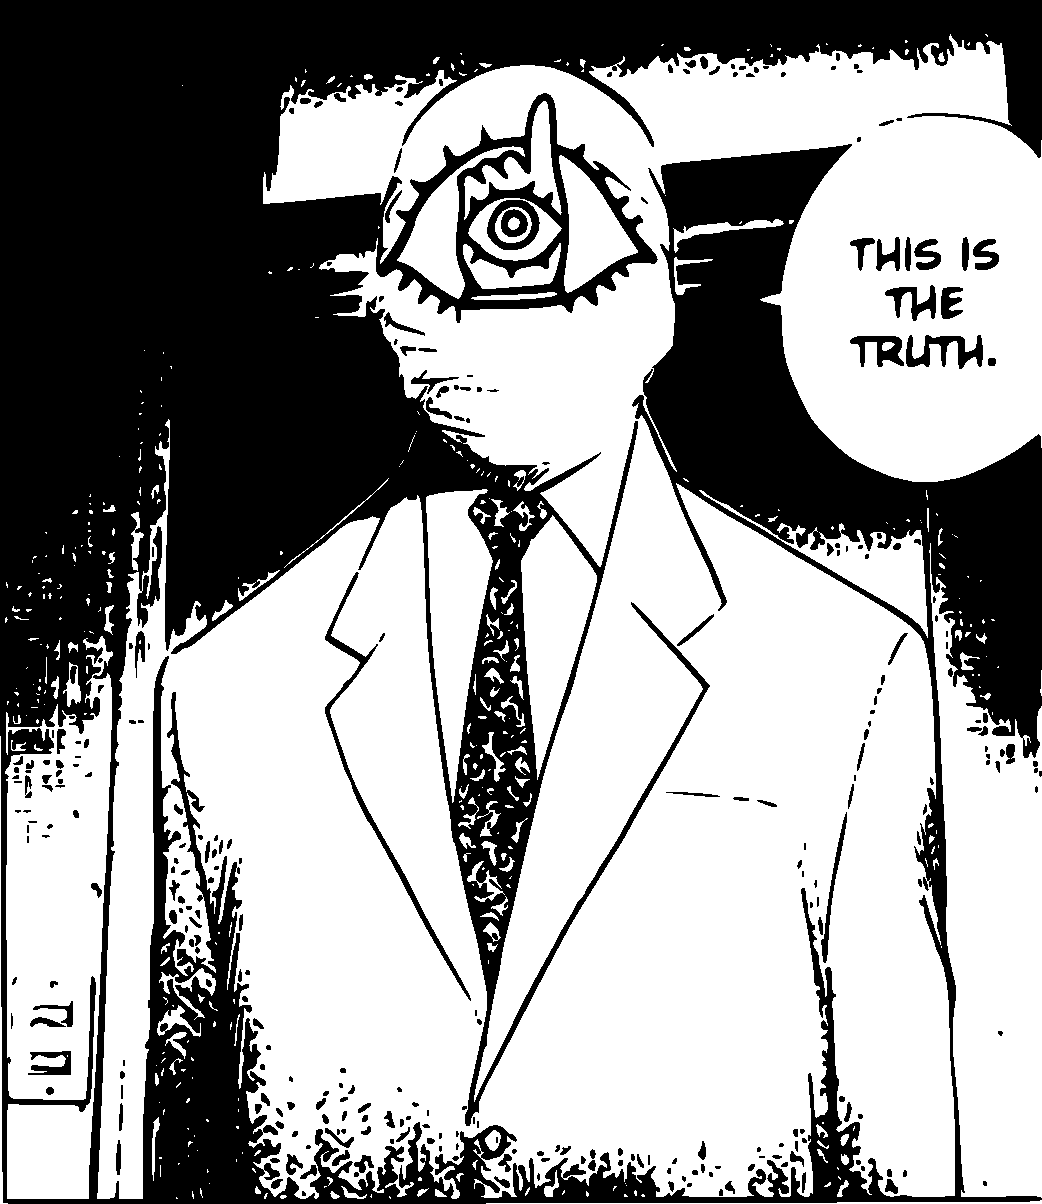
\includegraphics[width=0.4\textwidth,right ]{../../preamble/tomodachi.pdf} 
\end{figure}
\newpage %\setmainfont{Times New Roman}
\normalsize

\tableofcontents 
\newpage

%==================FOOTER e HEADER=======================%
\fancyhf{}
\fancyhead[L]{\nouppercase{\leftmark}}
\fancyhead[R]{Sezione \thesection}
\fancyfoot[C]{\thepage}
\fancyfoot[L]{\titolo}
\fancyfoot[R]{ Marco Casu}
%\fancyfoot[R]{\setmainfont{Palace Script MT}\huge Marco Casu \setmainfont{Times New Roman}}
%==================FOOTER e HEADER=======================%

\newtheorem{definition}{Definition}
\newtheorem{theorem}{Theorem}
%==================INIZIO======================%
\chapter{Introduction}
\section{Basic Definition of a ML Problem}
In this chapter we will introduce the basics of what is a machine learning problem, giving a mathematical definition. informally, with machine learning we define the use of knowledge (data) to improve the performance of a given program, using past experiences.\bigskip

Generally, we use machine learning to solve problems with no deterministic solutions, trying to find an approximate one (such as recognizing what animal is represented in a given photo).\bigskip 

Usually, a machine learning problem consists in three main component:\begin{itemize}
    \item $T$ : the given task
    \item $P$ : a performance metric
    \item $E$ : the past experiences (the data)
\end{itemize}
Let's see an example, we want to model a program capable of playing \textit{Checkers}.
\begin{center}
    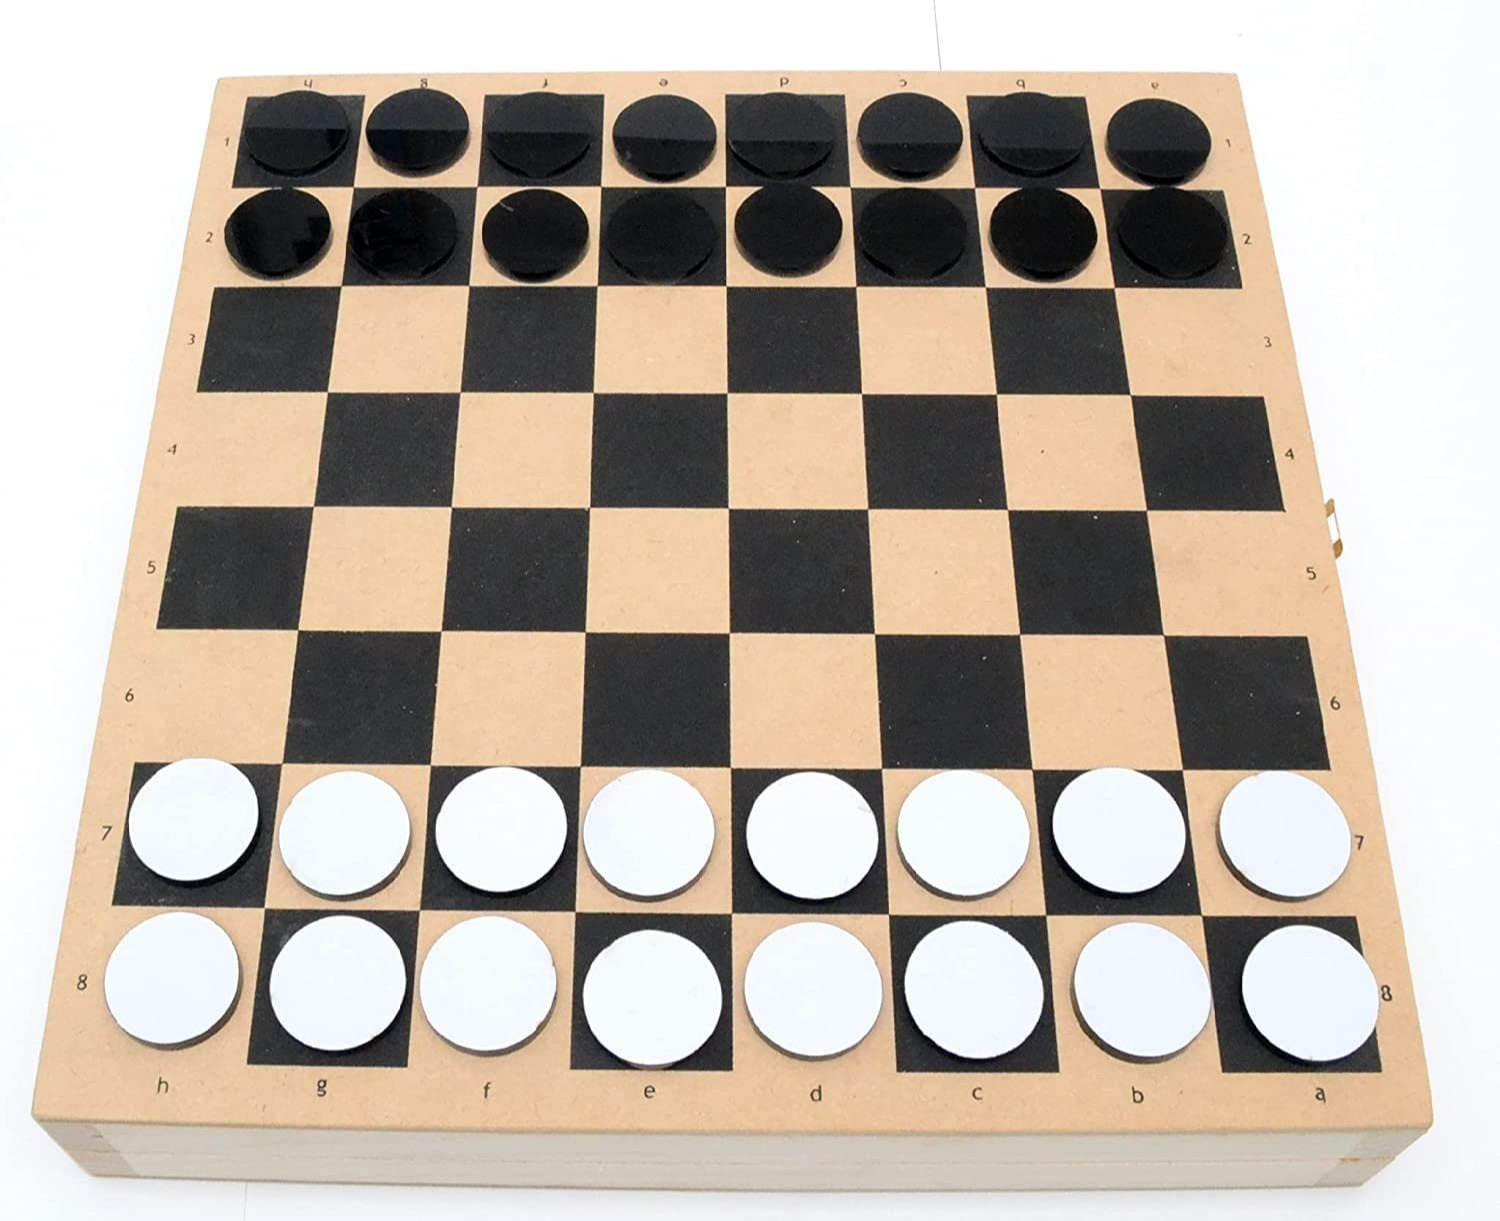
\includegraphics[width=0.35\textwidth]{images/Checkers.jpg}
\end{center}
The task $T$ is to play the game, the performance metric $P$ measure the ratio of win in a tournament, and the experiences is given by the past match. We can create this matches by letting the computer play against himself, or by making it play against a human. We can consider two types of target functions that models the behavior of the model:\begin{itemize}
    \item $ChooseMove : Board\rightarrow Move$
    \item $V : Board\rightarrow\R$
\end{itemize}
$Board$ is the set of the possible board configurations, move is the set of feasible moves. The image of the function $V$ should represents the validity of a board in the following sense:\begin{itemize}
    \item if $b\in Boards$ is a configuration that represents the win of the player, then $V(b)=1$
    \item else if $b\in Boards$ is a configuration that represents the win of the opponent, then $V(b)=-1$
    \item else if $b\in Boards$ is a configuration that represents a draw, then $V(b)=0$
    \item else, $V(b)=V(b')$ where $b'$ is
the best final board state that can be achieved starting from $b$ and
playing optimally until the end of the game.
\end{itemize}
The function $V$ can be used to predict the next move by considering all possible boards that can be obtained from the feasible moves.
We focus on the function $V$, this should be an optimal model, but is not computable, because we cannot tell if a play is ''optimal'' (this is the goal of the model), so we want to consider a function that approximate the behavior of $V$.\bigskip

We consider a function $\hat V: Board\rightarrow\R$ defined as follows:\begin{equation}
    \hat V(b)=\sum_{i=0}^6w_if_i(b)
\end{equation}
where $\mathbf w = (w_i)$ is real coefficients, and the functions $f_i$ represents some features of the given board:\begin{itemize}
    \item $f_1(b)$ : number of black pieces on $b$
    \item $f_2(b)$ : number of red pieces on $b$
    \item ecc...
\end{itemize}
We don't know if some features are useful to predict which move is optimal, is important that this features model the knowledge of the \textit{domain} (in this case, the game of Checkers). \bigskip

with \textit{learning the function} $\hat V$, we intend to finds the coefficients $\mathbf w$ which make the function $\hat V$ more similar to $V$ as possible. There are various method to find these coefficients.\bigskip

Let's introduce some notation:\begin{itemize}
    \item with $V$ we  define the \textbf{target function} (always unknown and uncomputable).
    \item with $\hat V$ we  define the \textbf{learned function}, the approximation of $V$ that we want to find.
    \item with $V_{train}(b)$ we define the value of $V$ obtained at $b$, where $b$ is a part of a data set that is given. We will use the values of $V_{train}$ on the data set to synthesize $\hat V$.
    \item with $D$ we define the given data set:\begin{equation}
        D=\bigcup_{i=1}^n\{(b_i,V_{train}(b_i))\}
    \end{equation}
    $n$ is the number of the available data.
\end{itemize}
The iterative method given in the Algorithm \ref{alg:LMS} is an informal example of how we can find the values for $\mathbf w$.
\begin{algorithm}
    \caption{LMS weight update rule}\label{alg:LMS}
    \begin{algorithmic}
    \Require $D$, $V_{train}$, $k$
    \State initialize $\mathbf w$ with small random values 
    \For{$k$ times}  
    \State select a sample $b$ from $D$
    \State $error(b)=V_{train}(b)-\hat V(b)$
    \For{each feature $i$} 
    \State $w_i\leftarrow w_i+c\cdot f_i(b)\cdot error(b)$
    \EndFor
    \EndFor
    \end{algorithmic}
\end{algorithm}
In this case $c$ is a small constant, usually in $(0,1]$, to moderate the rate of learning.\bigskip

The function $error(b)$ is computable only on the sample $b$ given in the dataset $B$, the goal of the method is to converge to a local minimum for the function  \begin{equation}
    \sum_{b_i\in D}error(b_i).
\end{equation}
Once we synthesize $\hat V$ with this method, we can make the model play against human and track the result to use it as an additional dataset. The diagram in image \ref{img:DesignChoice} represents the process of designing an artificial intelligence agent.

\begin{figure}[h!]
    \centering
    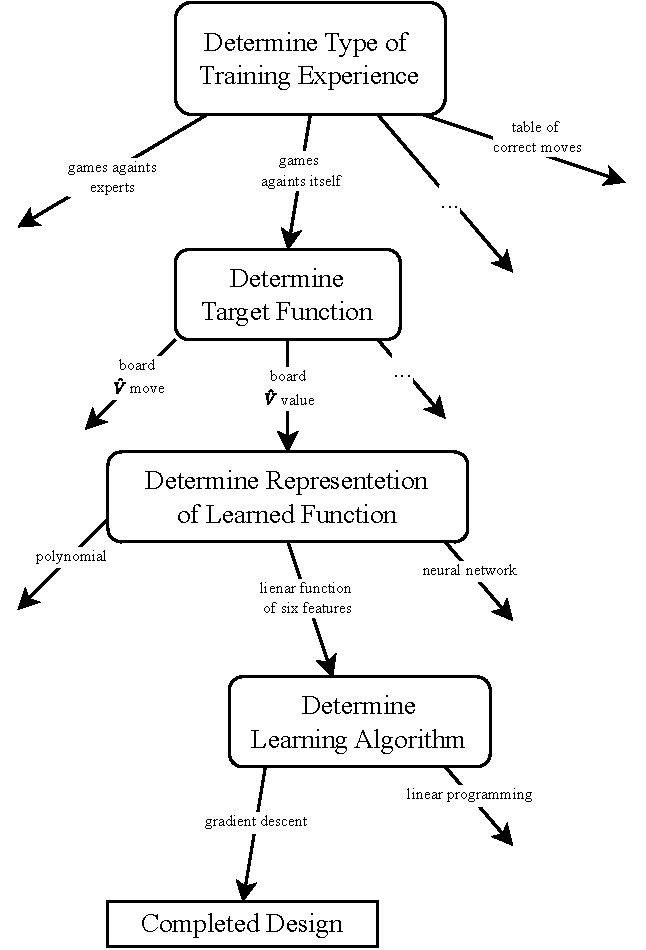
\includegraphics[width=0.35\textwidth]{images/DesignChoice.pdf}
    \caption{Design Choices}
    \label{img:DesignChoice}
\end{figure}
\section{Types of Machine Learning Problems}
There are different types of machine learning problems:\begin{itemize}
    \item Supervised Learning\begin{itemize}
        \item Classification
        \item Regression
    \end{itemize}
    \item Unsupervised Learning
    \item Reinforcement Learning
\end{itemize}

\begin{definition}
    Given a function $f:X\rightarrow Y$, and a training set $X_D\subset X$ containing information about $f$, \textbf{learning} the function $f$ means computing an approximated function $\hat f$ such that is much close as possible to $f$ on $X$\begin{equation}
        \hat f(x)\simeq f(x), \ \ x\in X.
    \end{equation}
\end{definition}
This is not a simple problem, $f$ is not computable, so the difference $f-\hat f$, and $X$ is usually uncountable ora big set, way bigger than the training set $X_D$. \bigskip

Machine learning problems can be classified in terms of the input data set $D$, given a target function $f:X\rightarrow Y$ a problem is\begin{itemize}
    \item a \textbf{supervised learning} problem if $D=\bigcup_{i=1}^n\{(x_i,y_i)\}\subset X\times Y$ .
    \item an \textbf{unsupervised learning} problem if $D=\bigcup_{i=1}^n\{(x_i)\}\subset X$.
    \item a \textbf{reinforcement learning} problem, the condition on the input dataset will be discussed later.
\end{itemize}
The problems can also be classified in terms of the target function $f:X\rightarrow Y$
\begin{align*}
   & X=\begin{cases}
        A_1\times \dots \times A_m, \ A_i \text{ finite set} \ \ \textbf{(Finite Discrete Problem)}\\ 
        \R^n \ \ \textbf{(Continuous)}
    \end{cases}\\ 
    & Y=\begin{cases}
         \R^k \ \ \textbf{(Regression)}\\ 
        \{C_1,C_2\times C_k\} \ \ \textbf{(Classification)}
    \end{cases}
\end{align*}
special case (\textbf{Concept Learning}):\begin{align*}
    & X = A_1\times \dots \times A_m, \ A_i \text{ finite set}\\ 
    & Y = \{0,1\}
\end{align*}
Classification problems is also known as \textit{Pattern Recognition Problems}, the goal is to return the class to which a specific instance belong.\begin{center}
     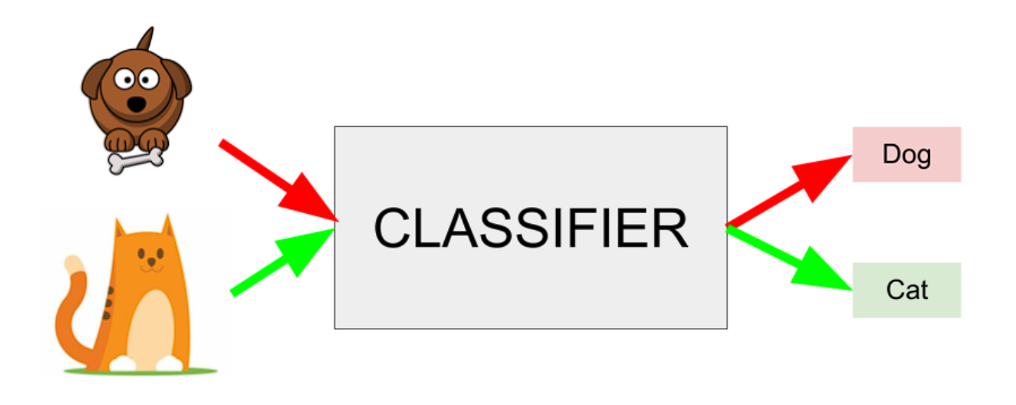
\includegraphics[width=0.6\textwidth]{images/classifier.png}
\end{center}
Some examples are:\begin{itemize}
    \item face/object/character recognition
    \item speech/sound recognition
    \item medical diagnosis
    \item document classification.
\end{itemize}
Regression problems consists in approximating real valued functions.
\begin{center}
     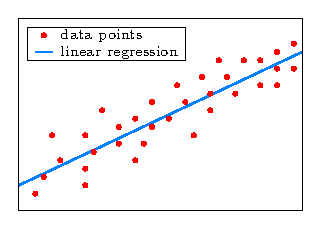
\includegraphics[width=0.35\textwidth]{images/regression.eps}
\end{center}
Unsupervised learning discovers data patterns without a specific output. The main goal is to understand what's normal in a dataset. \textit{Clustering} is a key technique that groups similar data points. Applications include customer segmentation, image compression, and bioinformatics motif learning.\bigskip

Reinforcement learning consists in learning a policy, which is a strategy that tells the agent what action to take in any given situation (or state) to maximize its long-term reward. This is often represented as a function that maps a state to an action. Unlike supervised learning, where the model is trained with labeled examples, in reinforcement learning agents learn through a process of trial and error.\bigskip

They don't have a correct answer to guide them. Instead, they receive sparse and time-delayed rewards. This means the feedback (the reward) for a good action might not come immediately, and it might be a simple, numerical value (like +1 for winning a game or -1 for losing). Some examples are:\begin{itemize}
    \item Game playing: Think of programs that have learned to play chess, Go, or video games better than humans.
    \item Robotic tasks: A robot learning to navigate a room, pick up an object, or perform a specific manufacturing task.
    \item Any dynamical system with an unknown or partially known model: This is a broad category that includes things like optimizing traffic flow, managing a power grid, or controlling financial trading strategies.
\end{itemize}
\begin{center}
     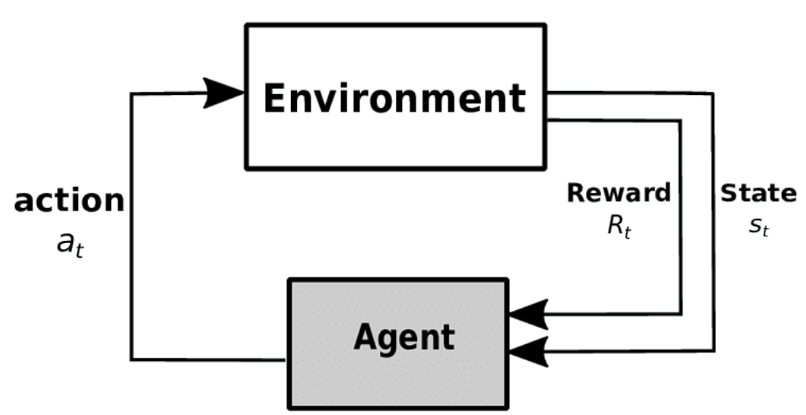
\includegraphics[width=0.35\textwidth]{images/RL_diagram.png}
\end{center}
In concept learning, the output consists in only two classes, the target function $c:X\rightarrow\{0,1\}$ maps  any kind of input in one of two distinct values. The following example model a program that predict if is a good day to play Tennis, the input set is $$ 
X=Day\times Outlook \times Temperature \times Humidity \times Wind 
$$
the output set is $PlayTennis=\{\text{Yes, No}\}$. An example of data samples:\begin{center}
\begin{tabular}{cccccc}
\toprule
$Day$ & $Outlook$ & $Temperature$ & $Humidity$ & $Wind$ & $PlayTennis$ \\
\midrule
D1 & Sunny & Hot & High & Weak & No \\
D2 & Sunny & Hot & High & Strong & No \\
D3 & Overcast & Hot & High & Weak & Yes \\
D4 & Rain & Mild & High & Weak & Yes \\
D5 & Rain & Cool & Normal & Weak & Yes \\
D6 & Rain & Cool & Normal & Strong & No \\
D7 & Overcast & Cool & Normal & Strong & Yes \\
D8 & Sunny & Mild & High & Weak & No \\
D9 & Sunny & Cool & Normal & Weak & Yes \\
D10 & Rain & Mild & Normal & Weak & Yes \\
D11 & Sunny & Mild & Normal & Strong & Yes \\
D12 & Overcast & Mild & High & Strong & Yes \\
D13 & Overcast & Hot & Normal & Weak & Yes \\
D14 & Rain & Mild & High & Strong & No \\
\bottomrule
\end{tabular}
\end{center}
\section{Performance Evaluation}
Usually, we call \textbf{Hypothesis} a possible learned function $h$, and we define $H$ as the \textbf{Hypothesis space}, such space contains all possible function that can be learnt (all possible approximation of the target function). In this terms, a learning problem is described as a search in the hypothesis space using the given dataset $D$, that aims to find the best possible approximation $h^*$:\begin{equation}\label{sol_hypothesis}
    h^*=\arg \max_{h\in H} Performance(h,D)
\end{equation} 
\subsection{Concept Learning}
We focus now on the concept learning (binary classification), let's consider a target function\begin{equation}
    c:X\rightarrow \{0,1\}
\end{equation}
let $D\subset \{X,Y\}$ to be the sample set\begin{equation}
    D=\bigcup_{i=1}^n\{(x_i,c(x_i))\}
\end{equation}
we denote $X_D$ the point of $X$ in the sample set. For now, we assume that the sample set does not have noise:\begin{itemize}
    \item noise dataset $D=\bigcup_{i=1}^n\{(x_i,c(x_i)+\varepsilon_i)\}, \ \ \varepsilon_i\in\R$
    \item perfect dataset $D=\bigcup_{i=1}^n\{(x_i,c(x_i))\}$
\end{itemize}
in general, the dataset is noisy. We want to find a function $\hat f$ that approximate $c$, as we just said, the hypothesis space $H$ is the set of all hypothesis $h$.\bigskip
Each hypothesis is a possible solution to the problem \eqref{sol_hypothesis},  it is possible to compare an hypothesis  $h$ with $c$ on a sample in $X_D$.
\begin{definition}
    Given a target function $c$ and a set of sample point $X_D$, an hypothesis $h$ is \textbf{consistent} if\begin{equation}
        h(x)=c(x), \ \ \forall x\in X_D.
    \end{equation}
\end{definition}
The \textbf{Version Space} $VS_{H,D}$ is the set of all consistent hypothesis:\begin{equation}
    VS_{H,D}=\{h \ : \ h(x)=c(x), \ \ \forall x\in X_D\}\subset H.
\end{equation}
A solution that does not lie in the version space is probably not a good solution.\bigskip 

Let's consider an example, let $c$ to be the following target function\begin{equation}
    c:\N\rightarrow\{-,+\}
\end{equation}
the dataset is\begin{equation}
    D=\{(1,+),(3,+),(5,+),(6,-),
    (8,-),(10,-)\}
\end{equation}
given the hypothesis space $H$, we consider four different hypothesis\begin{align*}
    &h_1(n)=+\iff n\text{ is odd}\\
    &h_2(n)=+\iff n\le 5\\
    &h_3(n)=+\iff n\text{ is either 1 or prime}\\
    &h_4(n)=+\iff n\in\{1,3,5\}
\end{align*}
if $n=11$ we have\begin{align*}
    &h_1(11)=+\\
    &h_2(11)=-\\
    &h_3(11)=+\\
    &h_4(11)=-
\end{align*}
we can't tell which of the four hypothesis is better than the others. Let's now consider a new hypothesis space $H'$, defined as the power set of $H$\begin{equation}
    H'=\mathcal P(H)=\{I \ : \ I\subseteq H\}
\end{equation}
The set $H'$ contains more information than $H$, let $\theta\in H'$, we define the value of $\theta$ on $x$ in a different way\begin{align}
    &\theta = \bigcup_i\{h_i\}\\
    &\theta(x)=\text{maj}\bigcup_i\{h_i(x)\}
\end{align}
where the function maj returns the element that is more frequent in a set. It's important to know that, if you have a set where two different items appear the exact same number of times, and no other item appears more often than either of them, then the majority element can't be identified, and the value of the function maj is undefined.\bigskip

With the hypothesis space $H'$, the point $n=11$ can't be classified\begin{equation}
    \theta(11)=\text{maj}\{h_1(11),h_2(11),h_3(11),h_4(11)\}=\text{maj}\{+,-,+,-\}.
\end{equation}
Even if $H'$ is more powerful than $H$, this hypothesis space can't classify an element that can be classified in $H$, this problem is called overfitting.\bigskip

Now let's consider the following target function\begin{equation}
    c:\N^2\rightarrow\{+,-\}
\end{equation}
with the following dataset $D$ that can be plotted on a 2D plane:\begin{center}
    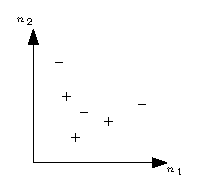
\includegraphics[width=0.25\textwidth]{images/N2_hypothesis_1.eps} 
\end{center}
We consider $H$ as the set of the functions that, assigns at all the points in a specific rectangle the $+$ value, and the $-$ value for all the points outside.
\begin{eqnarray*}
    h\in H \iff\Big( \exists R:=\{(x,y) \ : \ a\le x\le b\land c\le y\le d\} : h(x,y)=+\iff (x,y)\in R\Big )
\end{eqnarray*}
For that data samples, does not exists a consistent hypothesis, because does not exists a rectangle that contains all the $+$ value point, letting outside the $-$ value points.
\begin{center}
    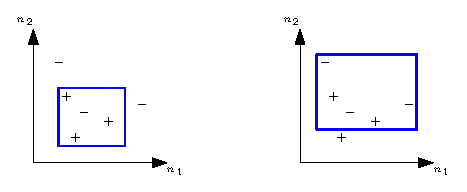
\includegraphics[width=0.6\textwidth]{images/N2_hypothesis_2.eps} 
\end{center}
If we consider the hypothesis space $H'=\mathcal P(H)$, geometrically, we can represent a function by a finite number of rectangles, in this case consistent hypothesis are allowed, but no $-$ value points can be predicted.
\begin{center}
    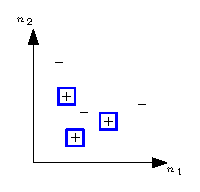
\includegraphics[width=0.25\textwidth]{images/N2_hypothesis_3.eps} 
\end{center}
Even in this example, a powerful representation of the hypothesis space lead to less generalization. This is known (as previously said) as \textbf{overfitting}, when the hypothesis space is not powerful enough, the problem could not be represented well, this is known as \textbf{underfitting}.\bigskip

If $n$ is a number that determines how big an hypothesis space, we can observe the following trend about the performance of a model.

\begin{figure}[h!]
    \centering
    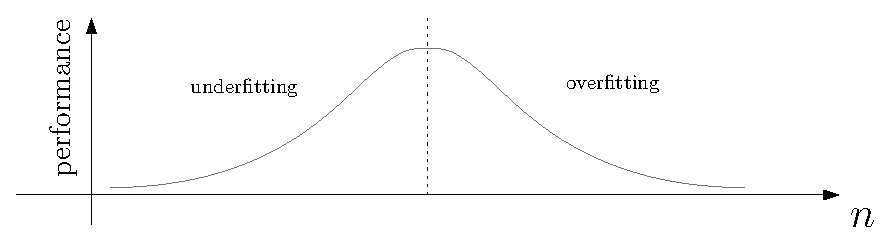
\includegraphics[width=0.65\textwidth]{images/fitting.eps}
    \caption{overfitting and underfitting trend}
    \label{img:fitting_trend}
\end{figure}

\subsection{Error Estimation and Performance Metric}
We want to define a metric for the performance of a model, to estimate how a given hypothesis $h$ is good respect to the others. We have to introduce some statistical methods, let's consider a target function\begin{equation}
    f:X\rightarrow Y
\end{equation}
where $Y$ is countable (classification problem). Let $\mathcal D$ to be a probability distribution over $X$.
\begin{definition}\label{def:prob_distr}
    If $X$ is a countable subset of $\R^n$, $\mathcal D$ is a probability distribution on $X$ if\begin{eqnarray}
        \forall x\in X, \ \ \mathcal D(x)\in [0,1]
    \end{eqnarray}
    and \begin{align*}
        &\sum_{x\in X}\mathcal D(x)=1 
    \end{align*}
    if $X$ is an uncountable subset of $\R^n$,  $\mathcal D$ is a probability distribution on $X$ if \begin{eqnarray}
        \forall x\in X, \ \ \mathcal D(x)\ge 0
    \end{eqnarray}
    \begin{align*}
        &\int_X\mathcal D(x)dx=1
    \end{align*}
\end{definition}
\begin{definition}
    Given a target function $f:X\rightarrow Y$, an hypothesis $h$ and a probability distribution $\mathcal D$ on $X$, the \textbf{true error} is the probability that $h$ will misclassify an instance $x\in X$ drawn according to the distribution $\mathcal D$:
    \end{definition}
    \begin{equation}
        \text{error}_{\mathcal D}(h)=
        \Prob_{x\sim \mathcal D}
        (f(x)\ne h(x)) 
    \end{equation}
\textbf{Note}: With $x\sim \mathcal D$, we mean that $x$ was extracted from $X$ according to the probability distribution $\mathcal D$. We remind that, if $\mathcal D(x)=p$, then, the probability of extracting $x$ from $X$ by taking a random element is $p$.\bigskip

Since we can't compute $f$ for all $x\in X$, the true error can't be computed. We need to define an estimation of the error given by the sample set extracted from $X$.
\begin{definition}
    Given a target function $f:X\rightarrow Y$, an hypothesis $h$ and a sample (finite) set $\mathcal S\subset X$, the  \textbf{sample error} is defined as follows:
\end{definition}\begin{equation}
        \text{error}_{\mathcal S}(h)=
        \frac{1}{|\mathcal S|}\sum_{x\in\mathcal S}\delta(f(x)\ne h(x))
\end{equation}
where\begin{itemize}
    \item $\delta(\phi)=1$ if $\phi$ is true
    \item $\delta(\phi)=0$ if $\phi$ is false.
\end{itemize}
The sample error can be computed since, for each $x\in\mathcal S$, we know the value of $f(x)$. Is an approximation of the true error that depends from the sample set $\mathcal S$.\bigskip

Since $\text{error}_{\mathcal S}(h)$ depends from the choice of $\mathcal S$, is not fixed, but we can model it as a random process, by extracting $n$ random values from $X$ according to the distribution $\mathcal D$ to construct $\mathcal S$, and we can evaluate the expected value of $\text{error}_{\mathcal S}(h)$ denoted \begin{equation}
    \VA(\text{error}_{\mathcal S}(h)).
\end{equation}
We want to formalize this expected value, in this case the sample error is a random variable that assign to each subset $\mathcal S$ of $X$ of size $n$ a number between 0 and $1$:
\begin{align}
    &\text{error}_{\mathcal S}(h) : \Omega \rightarrow [0,1]\\
    &\Omega =\{\mathcal S \ : \ \mathcal S \subset X \land |\mathcal S|=n\}
\end{align}
in this context, $n$ is fixed. The probability of getting a certain value $\gamma$ from this random variable, is the probability to extract from $X$ a subset $\mathcal S$ of $n$ items such that, the sample error is $\gamma$, and this depends from the probability distribution $\mathcal D$ on $X$. The expected value $\VA(\text{error}_{\mathcal S}(h))$ is now well defined.
\subsection{Unbiased Estimation}
\begin{definition}
    The \textbf{bias} is defined as the expected value of the difference between the sample error and the true error:
\end{definition}
    \begin{equation}
        \VA(\text{error}_{\mathcal S}(h))-\text{error}_{\mathcal D}(h).
    \end{equation}
We want to find an unbiased sample error, in such case:\begin{equation}
    \text{bias = 0} \implies \VA(\text{error}_{\mathcal S}(h))=\text{error}_{\mathcal D}(h)
\end{equation}
To compute an unbiased estimation, we need to train an evaluate an hypothesis $h$ on different set, let $D$ to be the dataset, we have to split $D$ in two disjoint set\begin{align}
    &D=T\cup S\\
    &T\cap S = \emptyset
\end{align}
Usually, $\frac{|T|}{|D|}\simeq \frac{2}{3}$.
We use $T$ to train our learning function to get $h$, and then, we calculate the sample error on $S$\begin{equation}
     \text{error}_{ S}(h)=
        \frac{1}{| S|}\sum_{x\in S}\delta(f(x)\ne h(x))
\end{equation}
is ideal to choose $T$ and $S$ such that they have similar probability distribution over the features, in this case the random variable $\text{error}_{ S}$ is an unbiased estimator for the true error $\text{error}_{ \mathcal D}$. 
\subsection{The Cross Validation Algorithm and others Performance Metrics}
There exists an algorithm to estimate the expected value of the sample error, more the dataset $D$ is large, more the estimation will be precise.
The algorithm \ref{alg:CrossVal} estimate the expected value of the error, with $L$ is denoted a fixed learning algorithm:\begin{itemize}
    \item $h=L(T)$, is the result of the learning algorithm $L$ applied on the training set $T$
\end{itemize}
\begin{algorithm}
    \caption{K-Fold Cross Validation}\label{alg:CrossVal}
    \begin{algorithmic}
    \Require $D$, $k$, $h$, $L$
    \State partition $D$ in $k$ disjoint sets $S_1,S_2\dots, S_k$
    \For{$i=1,2\dots,k$}
    \State $T_i\leftarrow  D\backslash S_i$
    \State $h_i\leftarrow L(T_i) $
    \State $\delta_i = \text{error}_{S_i}(h_i)$
    \EndFor
    \State\Return $\text{error}_{L,D}=\displaystyle\frac{1}{k}\sum_{i=1}^k\delta_i$
    \end{algorithmic}
\end{algorithm}
We define the accuracy of a learning algorithm $L$ as \begin{equation}
    \text{accuracy}=1-\text{error}_{L,D}.
\end{equation}
The cross-validation algorithm can be used to compare the accuracy of two different learning methods $L_a$ and $L_b$, as shown in algorithm \ref{alg:CrossVal_compare}.

\begin{algorithm}
    \caption{Accuracy Comparator}\label{alg:CrossVal_compare}
    \begin{algorithmic}
    \Require $D$, $k$, $h$, $L$
    \State partition $D$ in $k$ disjoint sets $S_1,S_2\dots, S_k$
    \For{$i=1,2\dots,k$}
    \State $T_i\leftarrow  D\backslash S_i$
    \State $h_a\leftarrow L_a(T_i) $
    \State $h_b\leftarrow L_b(T_i) $
    \State $\delta_i = \text{error}_{S_i}(h_a)-\text{error}_{S_i}(h_b)$
    \EndFor
    \State\Return $\bar\delta=\displaystyle\frac{1}{k}\sum_{i=1}^k\delta_i$
    \end{algorithmic}
\end{algorithm}

Now that we defined the sample error, we can give a formal definition of overfitting. Let $h$  to be an hypothesis for a model, $h$ is overfitting is exists an hypothesis $h'$ such that\begin{align}
    &\text{error}_{S}(h)<\text{error}_{S}(h') \\ &\land\\
    &\text{error}_{\mathcal D}(h)>\text{error}_{\mathcal D}
\end{align}

Let's consider other performance metrics in binary classification. Let $f:X\rightarrow\{-,+\}$ to be the target function ad let $D$ to be a sample set such that, $90\%$ of elements in $D$ is of class $+$. An hypothesis that always returns $+$ will have an accuracy of $90\%$, in this scenario the dataset is unbalanced, so the accuracy is not a good performance metric for the model. We can consider a table that counts the number of points in the sample set that are well classified or misclassified by an hypothesis:\begin{center}
    \begin{tabular}{c|cc|}
\cline{2-3}
                                 & \multicolumn{2}{c|}{predicted class}                 \\ \hline
\multicolumn{1}{|c|}{true class} & \multicolumn{1}{c|}{+}              & -              \\ \hline
\multicolumn{1}{|c|}{+}          & \multicolumn{1}{c|}{true positive}  & false negative \\ \hline
\multicolumn{1}{|c|}{-}          & \multicolumn{1}{c|}{false positive} & true negative  \\ \hline
\end{tabular}
\end{center}
we can define two additional metrics that is useful when we deal with binary classification:\begin{itemize}
    \item the \textbf{recall} is the ability of the hypothesis to avoid false negatives and is defined as follows\begin{equation}
        \frac{\text{true positive}}{\text{true positive}+\text{false negative}}
    \end{equation}
    \item the \textbf{precision} is the ability of the hypothesis to avoid false positives and is defined as follows\begin{equation}
        \frac{\text{true positive}}{\text{true positive}+\text{false positive}}
    \end{equation}
\end{itemize}
the importance of these metrics depend on the application.
\bigskip
\begin{figure}[h!]
    \centering
    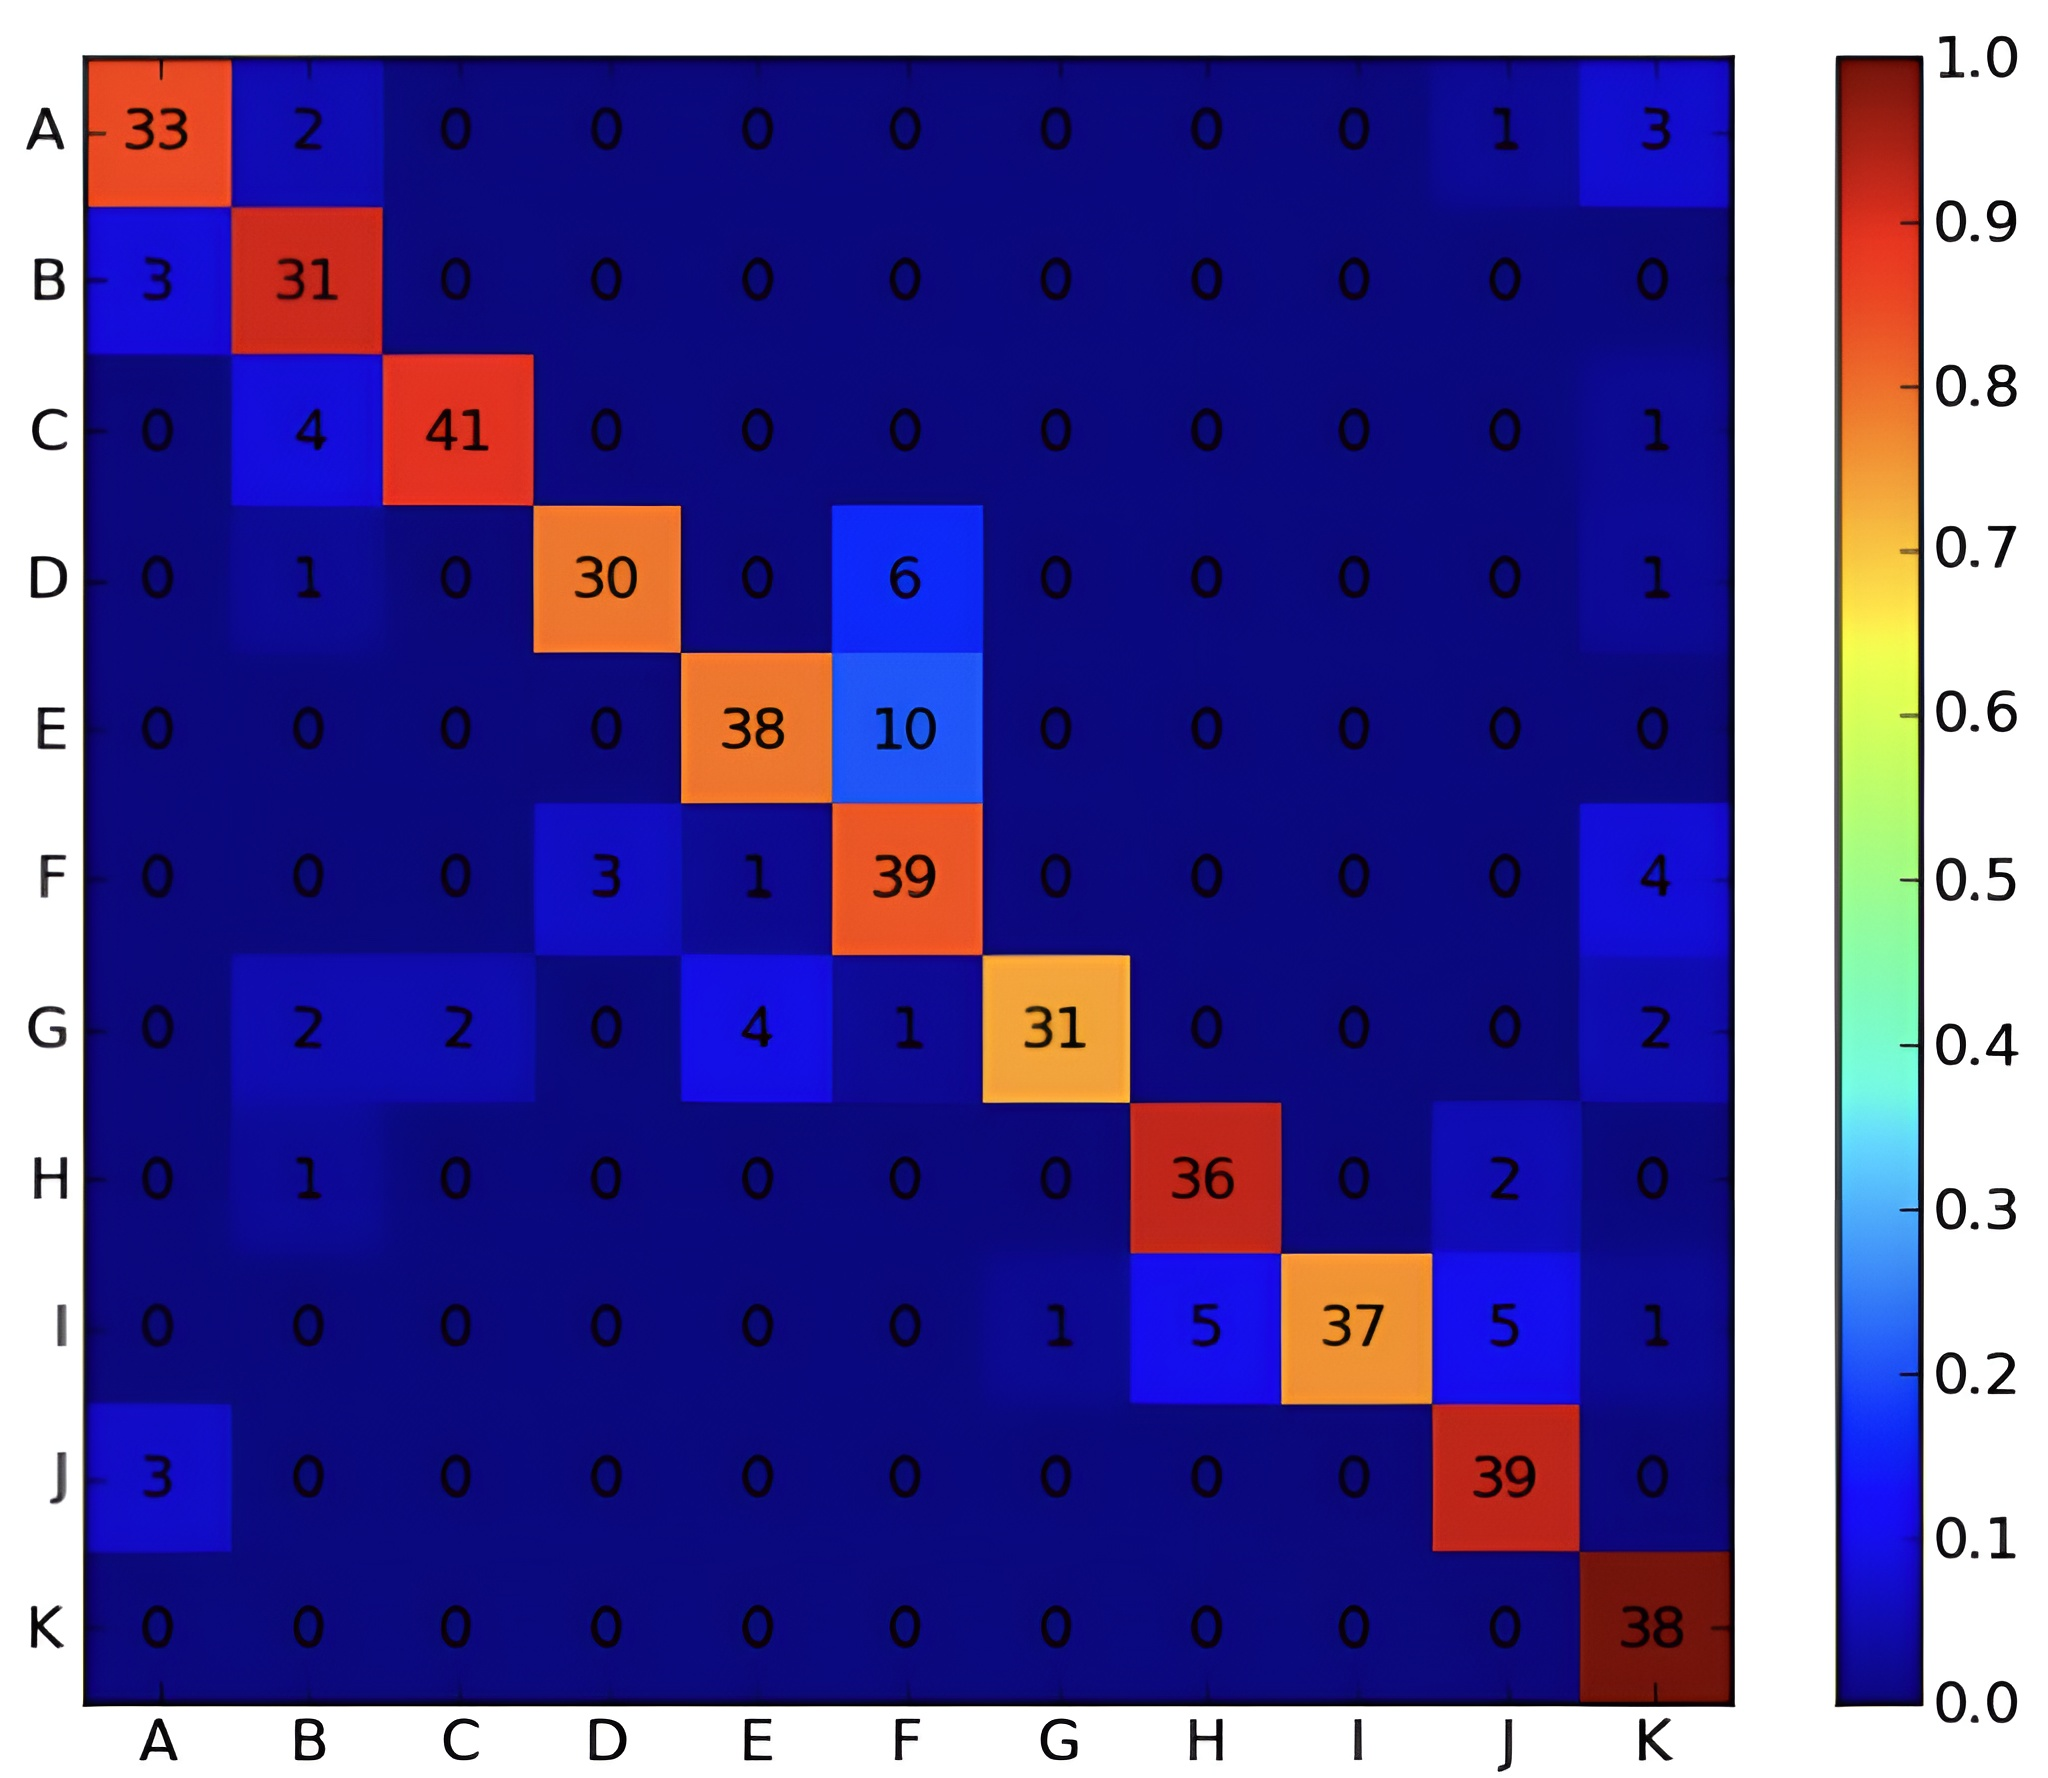
\includegraphics[width=0.3\textwidth]{images/conf_matrix.png}
    \caption{an example of a confusion matrix}
    \label{img:conf_matrix}
\end{figure}\bigskip

For the classification problems we can define an extension of the previous table, called \textbf{confusion matrix}, and report how many instances of class $C_i$ are classified in class $C_j$, the main diagonal contains the accuracy for each class. An example is shown in figure \ref{img:conf_matrix}.\bigskip

We consider now some performance metrics for the regression problems. Let $f:X\rightarrow\R^d$ to be the target function, and let $\hat f$ to be the learned function, for each sample $(x_i,f(x_i))$ in the dataset, we can compute the euclidian distance\begin{equation}
    |\hat f(x_i)-f(x_i)|.
\end{equation}
Let $n$ to be the number of samples, the three main metrics are the following:\begin{itemize}
    \item Mean Absolute Error\begin{equation}
        MAE=\frac{1}{n}\sum_{i=1}^n|\hat f(x_i)-f(x_i)|
    \end{equation}
    \item Mean Squared Error\begin{equation}
        MSE=\frac{1}{n}\sum_{i=1}^n(\hat f(x_i)-f(x_i))^2
    \end{equation}
    \item Root Mean Squared Error\begin{equation}
        RMSE=\sqrt{MSE}
    \end{equation}
\end{itemize}

The cross validation algorithm can be extended for the regression problems as shown in algorithm \ref{alg:CrossVal_regression}.

\begin{algorithm}
    \caption{K-Fold Cross Validation for Regression}\label{alg:CrossVal_regression}
    \begin{algorithmic}
    \Require $D$, $k$, $h$, $L$
    \State partition $D$ in $k$ disjoint sets $S_1,S_2\dots, S_k$
    \For{$i=1,2\dots,k$}
    \State $T_i\leftarrow  D\backslash S_i$
    \State $h_i\leftarrow L(T_i) $
    \State $\delta_i = MAE_{S_i}(h_i)$
    \EndFor
    \State\Return $\text{error}_{L,D}=\displaystyle\frac{1}{k}\sum_{i=1}^k\delta_i$
    \end{algorithmic}
\end{algorithm}
\chapter{Decision Trees}
Let's consider the following classification problem, we have a target function\begin{equation}
    c:X\rightarrow C
\end{equation}
and a data set \begin{equation}
    D=\bigcup_{i=1}^n\{(x_i,y_i)\}\subset X\times C
\end{equation}
our approach is to define the hypothesis space $H$ and search among all the possible solutions. Clearly we would like to find a solution $h^*\in D$ such that\begin{equation}
    h^*(x')\simeq f(x'), \ \ \forall x'\notin D.
\end{equation}
\textbf{Recall}: About the notation abuse, we say that $x'\in D$ if $\exists (x_i,y_i)\in D $ such that $x'=x_i$.\bigskip 

In this chapter we will see how to define the hypothesis space $H$ with \textit{decision trees}, let's assume that we are dealing with a finite problem, where \begin{equation}
    X=A_1\times \dots \times A_m \text{ with }A_i \text{ finite}
\end{equation}
and clearly $C$ is a finite set of classes.
\begin{definition}
    In the context of classification problems, a \textbf{decision tree} is a tree such that, each node is labeled with an attribute $A_i$, each edge is labeled with a value of an attribute $a_{i,j}\in A_i$, and each leaf assigns a classification value $c\in C$.
\end{definition}
A decision tree decides the class for each input $x\in X$, so we define the hypothesis space $H$ as the set of all possible decision trees.
The tree $h'$ showed in figure \ref{img:dec_tree}, defines the following value\begin{align}
    &h'(a_{1,4},a_{2,2},a_{3,2})=c_1
\end{align}
Let's consider the following example about tennis, the input space $X$ is\begin{align}
    &X = Outlook\times Temperature\times Humidity\times Wind\\
    &Outlook=\{sunny,overcast,rain\}\\
    &Temperature=\{hot,mild,cold\}\\
    &Humidity=\{normal,high\}\\
    &Wind=\{weak,strong\}
\end{align}
the target function $PlayTennis:X\rightarrow\{Yes,No\}$ should decides if the conditions are feasible to play tennis outside. The dataset is the onw shown in table \ref{tab:tennis_data_big}.
\begin{table}[h]
    \centering
    \caption{Dataset for the tennis problem}
    \label{tab:tennis_data_big}
\begin{tabular}{cccccc}
\toprule
$Day$ & $Outlook$ & $Temperature$ & $Humidity$ & $Wind$ & $PlayTennis$ \\
\midrule
D1 & Sunny & Hot & High & Weak & No \\
D2 & Sunny & Hot & High & Strong & No \\
D3 & Overcast & Hot & High & Weak & Yes \\
D4 & Rain & Mild & High & Weak & Yes \\
D5 & Rain & Cool & Normal & Weak & Yes \\
D6 & Rain & Cool & Normal & Strong & No \\
D7 & Overcast & Cool & Normal & Strong & Yes \\
D8 & Sunny & Mild & High & Weak & No \\
D9 & Sunny & Cool & Normal & Weak & Yes \\
D10 & Rain & Mild & Normal & Weak & Yes \\
D11 & Sunny & Mild & Normal & Strong & Yes \\
D12 & Overcast & Mild & High & Strong & Yes \\
D13 & Overcast & Hot & Normal & Weak & Yes \\
D14 & Rain & Mild & High & Strong & No \\
\bottomrule
\end{tabular}
\end{table}

\begin{figure}[h!]
    \centering
    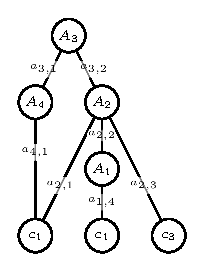
\includegraphics[width=0.25\textwidth]{images/decision_tree.eps}
    \caption{Example of a decision tree}
    \label{img:dec_tree}
\end{figure}

\begin{center}
	\begin{tabular}{>{\centering\arraybackslash}m{3in}>{\arraybackslash}m{3in}}
        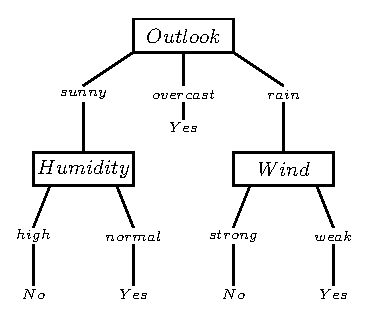
\includegraphics[width=0.3\textwidth ]{images/tennis_tree.eps} & Here's an example of a decision tree for the tennis problem. This representation is easy to classify a new instance that are not in the dataset, this tree defines rules such as: If the outlook is $overcast$, the output is $Yes$. The policy and the decisions are \textit{explicit}, and provides an explanation for the outcomes.
		\\
	\end{tabular}
\end{center}

In the hypothesis space $H$ we have all possible decision trees, that are finite for this kind of problems. Decision trees represent a disjunction of conjunctions of constraints, that can be easily described by looking at the tree, traveling the traces of the tree backward starting from the outcomes. An example is shown in figure \ref{img:conj_tree}. The recursive algorithm \ref{alg:dec_tree} works to compute one decision tree given the dataset $D$.\bigskip

\begin{figure}[h!]
    \centering
    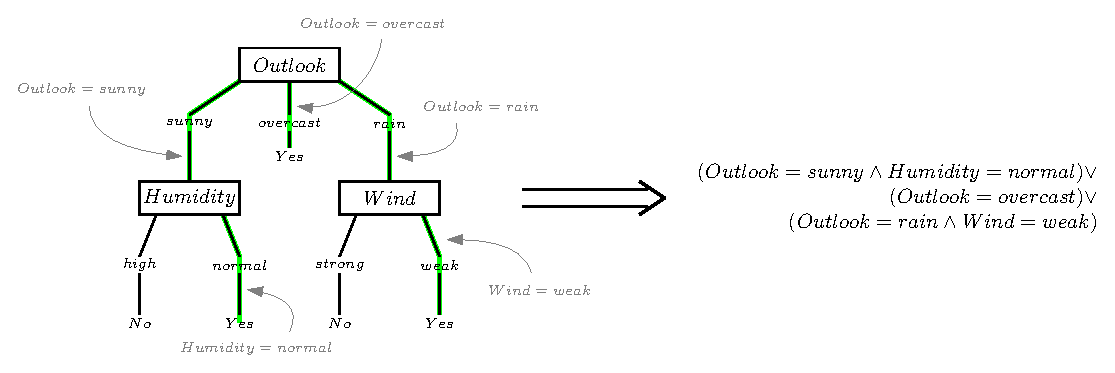
\includegraphics[width=1\textwidth]{images/conj_tree.eps}
    \caption{How paths in the tree transform into a logical formula}
    \label{img:conj_tree}
\end{figure}

\begin{algorithm}
    \caption{Computing Decision Tree for Binary Classification}\label{alg:dec_tree}
    \begin{algorithmic}
    \Require $D=\{(x_i,c_i)_i\}$, $Att=\{A_1\dots,A_m\}$
    \If{$\forall (x_i,c_i)\in D, \ \ c_i=+$}
    \State\Return $N(+)$
    \EndIf
    \If{$\forall (x_i,c_i)\in D, \ \ c_i=-$}
    \State\Return $N(-)$
    \EndIf
    \If{$Att=\emptyset$}
    \State $D_+=\{(x_i,c_i)\in D \ : \ c_i=+\}$
    \State $D_-=D\backslash D_+$
    \If{$|D_+|>|D_-|$}
    \State\Return  $N(+)$
    \EndIf
    \If{$|D_-|>|D_+|$}
    \State\Return  $N(-)$
    \EndIf
    \State\Return a random choice between $N(+)$ and $N(-)$
    \EndIf
    \State $A_i = \texttt{criteria}(Att)\in Att$
    \State we create a node $N(A_i)$
    \For{each $a_{i,j}\in A_i$}
    \State create an edge $N(A_i)\longrightarrow_{a_{i,j}} N(\ )$
    \State $D'=\{(x_i,c_i)\in D \ : \ x_i(A_i)=a_{i,j} \}$
    \State $N(\ )=$RecursiveCall($D',Att\backslash\{A_i\}$)
    \EndFor
    \State\Return the tree with root $N(A_i)$
    \end{algorithmic}
\end{algorithm}

We denote $N(+)$ a leaf node with the positive value, and $N(-)$ a leaf node with the negative value. If $A_i$ is an attribute, we denote $N(A_i)$ an intermediate node with the attribute $A_i$. We denote $N(\ )$ a node for which a value has not yet been assigned.

\section{The Information Gain}
The function \texttt{criteria}$(Att)$ choose one attribute from the remaining ones in the set $Att$, and defines decision policy. What is the best attribute to choose during the algorithm? That procedure defines the behavior of the algorithm. Let's consider the following example for a reduced version of the tennis problem, with the dataset shown in table \ref{tab:tennis_data}.

\begin{table}[h]
    \centering
    \caption{Dataset for the reduced tennis problem}
    \label{tab:tennis_data}
    \begin{tabular}{|c|c|c|c|}
        \hline
        {$Day$} & {$Outlook$} & {$Temperature$} & {$PlayTennis$} \\
        \hline
        D1 & Sunny & Hot & Yes \\
        \hline
        D2 & Sunny & Cold & Yes \\
        \hline
        D3 & Rain & Hot & No \\
        \hline
        D4 & Rain & Cold & No \\
        \hline
    \end{tabular}
\end{table}

If we apply the algorithm on this sample, there will be two possible solutions, one for the case where we choose $Outlook$ as the first choice for an attribute, one if we choose $Temperature$, the resulting trees as shown in figure \ref{img:tennis_criteria}.

\begin{figure}[h!]
    \centering
    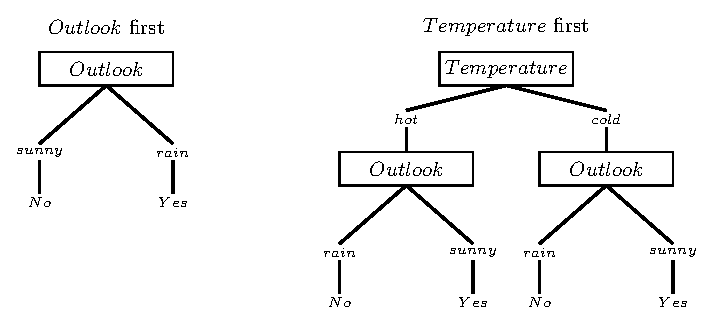
\includegraphics[width=0.7\textwidth]{images/tennis_criteria.eps}
    \caption{Different decision trees}
    \label{img:tennis_criteria}
\end{figure}

In general, not making the correct choice in the attributes can lead to a tree that incapsulate less information.  \begin{definition}
    Given an example dataset $S$, let $p_\oplus$ to be the proportion of positive examples in $S$, and $p_\ominus=1-p_\oplus$  the proportion of negative examples in $S$, the \textbf{entropy} of $S$ is the following value\begin{equation}
        Entropy(S)=-p_\oplus\log_2p_\oplus-p_\ominus\log_2p_\ominus.
    \end{equation}
\end{definition}
The curve of the $Entropy$ function is shown in figure \ref{fig:entropia_binaria}.
\begin{figure}[h!]
    \centering
    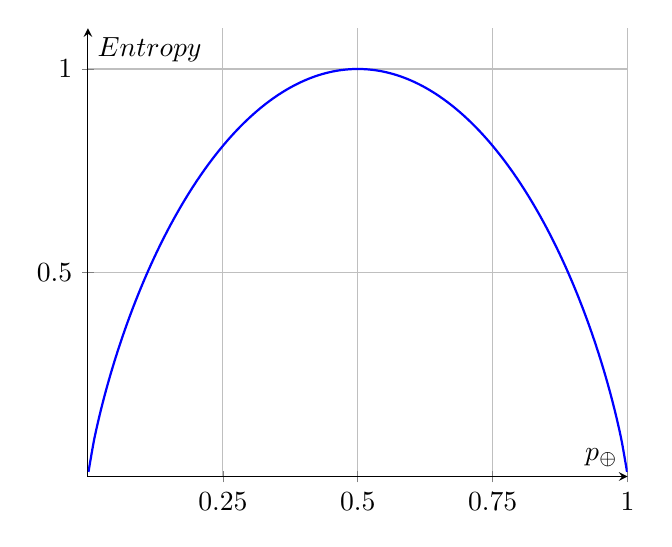
\begin{tikzpicture}
        \begin{axis}[
            % Impostazioni del grafico
            xlabel={$p_\oplus$},
            ylabel={$Entropy$},
            xmin=0, xmax=1, % Dominio della funzione
            ymin=0, ymax=1.1, % Imposta un intervallo comodo per l'asse Y
            grid=both, % Mostra la griglia
            axis lines=middle, % Assi centrati
            xtick={0, 0.25, 0.5, 0.75, 1},
            ytick={0, 0.5, 1},
            domain=0.001:0.999, % Evita x=0 e x=1, dove log è indefinito
            samples=100, % Numero di punti per una curva più liscia
        ]
        \addplot[
            blue, 
            thick, 
            smooth
        ] 
        {
            -(x * (ln(x) / ln(2))) 
            - ((1-x) * (ln(1-x) / ln(2)))
        };
        \end{axis}
    \end{tikzpicture}
    \caption{The curve of the $Entropy$ function}
    \label{fig:entropia_binaria}
\end{figure}

The entropy is minimum if we have all positive samples or all negative samples. The goal is to reduce the entropy of a dataset. We can partition the dataset in function of the different attributes, and then calculate the entropy for all the partitions. \bigskip

Given the table \ref{tab:tennis_data}, we can create two partitions, one by selecting $Outlook$, and one by selecting $Temperature$, as shown in figure \ref{img:partitions}.

\begin{figure}[h!]
    \centering
    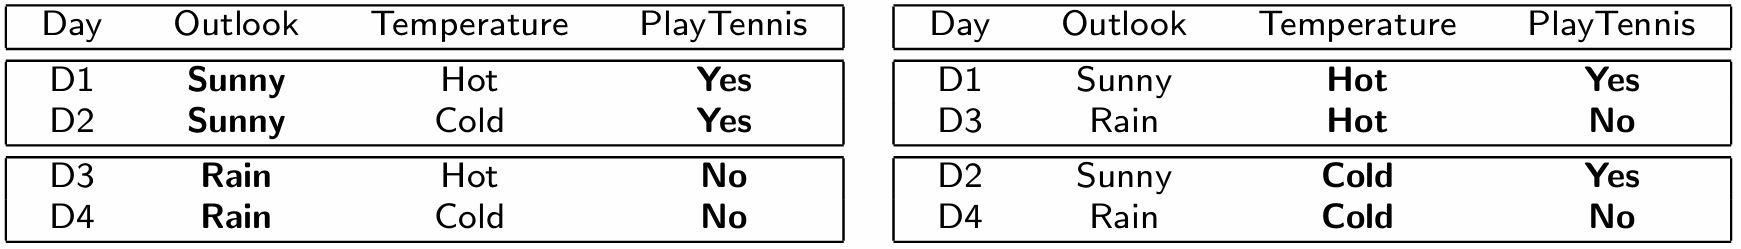
\includegraphics[width=0.9\textwidth]{images/partitions.png}
    \caption{Partitions of the dataset}
    \label{img:partitions}
\end{figure}

Splitting the dataset with outlook will generate two subsets with all positive/negative examples, so this two subsets will have an entropy of zero. In the other case, with temperature, the entropy will be 1.\bigskip

\noindent In the case of multi-valued target function (classification problem that is not binary), we can define the proportion of each class, denoted $p_i$, with $n$ classes, the entropy is\begin{equation}
    Entropy(S)=\sum_{i=1}^n-p_i\log_2p_i.
\end{equation}
\textbf{Note}: We define $0\log_20=0$.
\begin{definition}
    Given an example set $S$ and an attribute $A$, we define the \textbf{information gain} as the expected reduction in entropy of $S$ caused by knowing the value of the attribute $A$\begin{equation}
        Gain(S,A)=Entropy(S)-\sum_{v\in A}\frac{|S_v|}{|S|}Entropy(S_v)
    \end{equation}
    where\begin{equation}
        S_v=\{s\in S \ : \ s(A)=v\}
    \end{equation}
\end{definition}

If we take in example the dataset in the table \ref{tab:tennis_data_big}, we see that it have 9 positive samples and 5 negative samples, the entropy of the set is \begin{equation}
    -\frac{9}{14}\log_2\left(\frac{9}{14}\right)-\frac{5}{14}\log_2\left(\frac{5}{14}\right)=0.94   
\end{equation}
We want to calculate the information gain for the attribute $Wind$, that can be $Weak$ or $Strong$. If we partition the sub-dataset for this attribute, we get one dataset with 6 positive values and 2 negative values, and a sub-dataset with 3 positive values and 3 negative values.

\begin{table}[h]
    \centering
    \caption{Split Dataset for the tennis problem}
    \label{tab:tennis_data_big_split}
\begin{tabular}{cccccc}
\toprule
 $Outlook$ & $Temperature$ & $Humidity$ & \textbf{Wind} & $PlayTennis$ \\
\midrule
 Sunny & Hot & High & Weak & No \\
Overcast & Hot & High & Weak & Yes \\
 Rain & Mild & High & Weak & Yes \\
 Rain & Cool & Normal & Weak & Yes \\
 Sunny & Mild & High & Weak & No \\
 Sunny & Cool & Normal & Weak & Yes \\
 Rain & Mild & Normal & Weak & Yes \\
 Overcast & Hot & Normal & Weak & Yes \\

\bottomrule
\end{tabular}
\begin{tabular}{cccccc}
\toprule
 $Outlook$ & $Temperature$ & $Humidity$ & \textbf{Wind} & $PlayTennis$ \\
\midrule
Sunny & Hot & High & Strong & No \\
 Rain & Cool & Normal & Strong & No \\
 Overcast & Cool & Normal & Strong & Yes \\
 Sunny & Mild & Normal & Strong & Yes \\
 Overcast & Mild & High & Strong & Yes \\
Rain & Mild & High & Strong & No \\
\bottomrule
\end{tabular}
\end{table}

we have that\begin{align}
    &|S_{weak}|=8\\
     &|S_{strong}|=6\\
     &|S|=14\\
     &Entropy(S_{weak})=0.811\\
     &Entropy(S_{strong})=1
\end{align}
The information gain is\begin{align}
    &Gain(S,Wind)=Entropy(S)-\frac{8}{14}Entropy(S_{weak})-\frac{6}{14}Entropy(S_{strong})\\
    &=0.94-\frac{8}{14}0.811-\frac{6}{14}=0.048.
\end{align}

This is a little information gain. A possible criteria for the choice of the next attribute in the algorithm \ref{alg:dec_tree}, is to select the attribute with the highest information gain, in the case of the dataset \ref{tab:tennis_data_big}, we have that\begin{align}
    &Gain(S,Outlook)=0.245\\
     &Gain(S,Humidity)=0.151\\
      &Gain(S,Wind)=0.048\\
       &Gain(S,Temperature)=0.029
\end{align}

\noindent We call \texttt{ID3} the decision tree algorithm \ref{alg:dec_tree} with the information gain criteria. This algorithm can be seen as an algorithm that makes a search in the space of all possible hypothesis/decision trees.

The hypothesis space of decision trees is \textit{complete}, and we can represent all possible subsets of the input space. The algorithm returns one single hypothesis that is consistent with the dataset, this algorithm cannot find the global optimum function but a local minima.

This algorithm is not incremental and uses all the training set at each step.
\section{Issues in Decision Trees}
We have to consider the following problems:\begin{itemize}
    \item determining how deeply to grow the decision tree
    \item handling continuous attributes
    \item choosing appropriate attribute selection rule 
    \item handling training data with missing attribute values 
    \item handling attribute with different ''cost''.
\end{itemize}

\noindent Let $D$ to be the dataset shown in table \ref{tab:tennis_data_big}, we consider \begin{equation}
    D'=D\cup \left\langle  sunny,hot,normal,strong, PlayTennis=No\right\rangle
\end{equation}

\noindent\texttt{ID3} will generate two different decision trees $T,T'$ for the different dataset $D,D'$. The question is:\begin{quote}
    is $T'$ in general a better solution for this learning problem?
\end{quote}

In the general case, we have a dataset $D$ containing noisy data, and two decision trees $T$ and $T'$ obtained with different configurations of an \texttt{ID3}-like algorithm, where\begin{equation}
    accuracy_D(T')>accuracy_D(T)
\end{equation}
we don't know if $T'$ is a better solution, we should check the condition on a test set $S$\begin{equation}
    accuracy_S(T')>accuracy_S(T).
\end{equation}
Generally, the trend in figure \ref{img:trees_overfitting} is observed.\bigskip

\begin{figure}[h!]
    \centering
    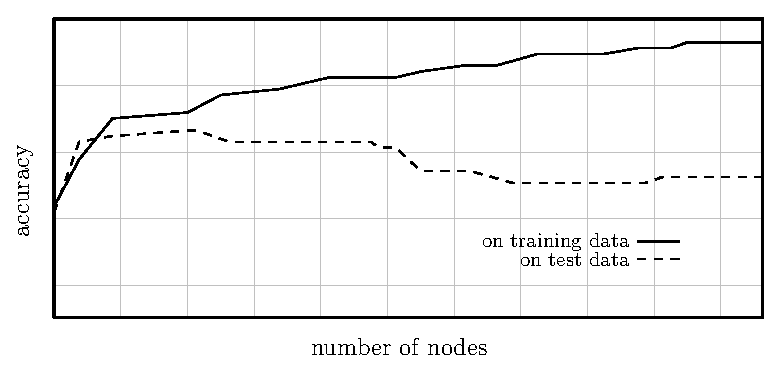
\includegraphics[width=0.7\textwidth]{images/trees_overfitting.eps}
    \caption{Decision trees overfitting}
    \label{img:trees_overfitting}
\end{figure}


To avoid overfitting, we should stop to grow the tree when the data split is not statistically significant, or could grow a full tree and then apply the \textit{post-prune}. With \textbf{pruning} we define the replacement of a sub-tree with a leaf node labelled as the most common class among samples filtered to the node.\bigskip

\begin{algorithm}
    \caption{Post Pruning}\label{alg:pruning}
    \begin{algorithmic}
    \Require a dataset $D$
    \State split data set in training $D_T$ and validation $D_V$
    \State generate a tree $T$ using the data set $D_T$
    \While{accuracy is not decreasing}
    \State  Evaluate the impact of pruning each node on the validation set 
    \State Greedily remove the one that most improves validation on accuracy
    \EndWhile
    \end{algorithmic}
\end{algorithm}

If the dataset is limited, reducing the set of training examples (used
as validation examples) can give bad results.\bigskip

Decision trees can be expanded to \textit{continuous values}, for example, if temperature is expressed in degrees, we could introduce a variation of the tree that will generate some ''test'' in terms of intervals\begin{itemize}
    \item $Temperature=82.5$
    \item $(Temperature > 72.3) = True,False$
\end{itemize}
So this decision trees will have tests on equalities and tests on real values. There are also several other ways of defining the criteria for selecting the best attributes to include as a node, there are other measures than the information gain. We cannot say that one is always better, it depends on the problem.\bigskip 

A dataset may have some samples with \textit{missing} attributes, for example:\begin{center}
    \begin{tabular}{|c|c|c|c|}
        \hline
        {$Day$} & {$Outlook$} & {$Temperature$} & {$PlayTennis$} \\
        \hline
        D1 & Sunny & UNKNOWN & Yes \\
        \hline
        D2 & Sunny & UNKNOWN & Yes \\
        \hline
        D3 & UNKNOWN & Hot & No \\
        \hline
        D4 & Rain & Cold & No \\
        \hline
    \end{tabular}
\end{center}
in such case, with decision trees we can use the samples by adding some information to replace the missing values\begin{itemize}
    \item If a node $n$ tests an attribute $A$, we assign the most common value of $A$ among other examples sorted to node $n$.
    \item We can assign the most common value for $A$ among the other examples with the same target value.
\end{itemize}
There are other algorithms based on decision trees:\begin{itemize}
    \item we can generate a set of decision trees (called \textbf{forest}) with some random criteria and integrates their values into a final result.
    \item that integration of result could occur as a majority vote (most common class returned by all the trees)
    \item random forest are less sensitive to overfitting.
\end{itemize}

\chapter{Probabilistic Models}
\section{Probability Recap}
Consider the following action\begin{equation}
    A_t=\text{ leave the house $t$ minutes before the flight}
\end{equation}
If we apply this action, what will be the answer to the question\begin{quote}
    The action $A_t$ will it get me there on time?
\end{quote}
The answer can't be a simple \textit{Yes} or \textit{No}, because depends from a series of casual factors that are unpredictable (such as the traffic reports, or a possible flat tire). The probability is needed to represents the uncertainties:\begin{itemize}
\item Given the available evidence, $A_{25}$ will get me at the airport on time with
probability 0.04
 \item Given the available evidence, $A_{60}$ will get me at the airport on time with
probability 0.84
 \item Given the available evidence, $A_{1440}$ will get me at the airport on time with
probability 0.999.
\end{itemize}
In this context, the set of \textit{all possible elementary events} that can occurs is called \textbf{Sample Space}, and is usually denoted $\Omega$.
\begin{definition}
    A \textbf{Discrete Probability Space} is a tuple $(\Omega,\mathcal A,\Prob)$ where\begin{itemize}
        \item $\Omega$ is the sample set of the elementary events.
        \item $\mathcal A\subseteq\mathcal P(\Omega)$ is a $\sigma$-algebra, and contains all the events that can occurs, for which we can calculate a probability. $\mathcal A$ satisfies the following properties:\begin{itemize}
            \item $\Omega\in\mathcal A$
            \item $A\in\mathcal A\implies A^C=\Omega\backslash A\in \mathcal A$
            \item if $\{A_i\}\subset\mathcal A$ is a countable sequence of events, then $\bigcup_i\{A_i\}\in\mathcal A$.
        \end{itemize}
        \item $\Prob$ is the \textbf{probability measure}, is a function $\Prob:\mathcal A\rightarrow[0,1]$ that assigns a probability to each event in $\mathcal A$ and satisfies the following properties:\begin{itemize}
            \item $\Prob(\Omega)=\displaystyle\sum_{\omega\in\Omega}\Prob(\{\omega\})=1$
            \item if $\{A_i\}$ is a countable collection of disjoint sets in $\mathcal A$, then\begin{equation}
                \Prob\left(\bigcup_{i}A_i\right)=\sum_i\Prob(A_i).
            \end{equation}
        \end{itemize}
    \end{itemize}
\end{definition}
\begin{definition}
    Given a probability space $(\Omega,\mathcal A,\Prob)$, a \textbf{random variable} is a function $X:\Omega\rightarrow Y$.
\end{definition}
The probability $\Prob$ induces a \textit{probability distribution} on a random variable $X$:\begin{equation}
    \Prob(X=x_i)=\sum_{\omega\in\Omega \ : \ X(\omega)=x_i}\Prob(\omega).
\end{equation}
\begin{definition}
    Given a probability space $(\Omega,\mathcal A,\Prob)$ a \textbf{proposition} $a$ is an event in $\mathcal A$, associated with a random variable $A:\Omega\rightarrow\{True,False\} $ such that\begin{equation}
        a := A \text{ is } True := \{\omega\in\Omega \ : \ A(\omega)=True\}.
    \end{equation}
\end{definition}
We can use the first order logic to combine and operates on propositions\begin{align}
    &\lnot a := A \text{ is } False := \{\omega\in\Omega \ : \ A(\omega)=False\}\\
    &a\land b := A \text{ and } B \text{ is } True :=\{\omega\in\Omega \ : \ A(\omega)=B(\omega)=True\}\\
    &\lnot a\lor b := A \text{ is }False\text{ or } B \text{ is } True :=\{\omega\in\Omega \ : \ A(\omega)=False\lor B(\omega)=True\}
\end{align}
Since a proposition is an element of $\mathcal A$, we can calculate the probability:\begin{equation}
    \Prob(\lnot a\lor b)=\sum_{\omega\in\Omega \ : \ A(\omega)=False\lor B(\omega)=True}\Prob(\omega)
\end{equation}
The Definition \ref{def:prob_distr} refers to a probability distribution, if $X:\Omega\rightarrow Y$ is a random variable, the probability distribution $\mathcal D$ assigns a probability to each element in $\mathcal P(Y)$.\bigskip

We will give now an example of a probability space. Let's consider the rolling of a dice, in this case we have\begin{itemize}
    \item the sample set $\Omega=\{1,2,3,4,5,6\}$
    \item the $\sigma$-algebra $\mathcal A = \{\{1\},\{1,2\}\dots\}$
    \item the probability $\Prob$ defined as follows\begin{equation}
        \forall\omega\in \Omega, \ \Prob(\{\omega\})=\frac{1}{6}.
    \end{equation}
\end{itemize}
The probability of getting an odd number is\begin{equation}
    \Prob(\{1,3,5\})=\Prob(\{1\})+\Prob(\{3\})+\Prob(\{5\})=\frac{1}{2}
\end{equation}
Let's consider the following random variable\begin{align}
    &X:\Omega\rightarrow\{-20,30\}\\
    &X(\omega)=30\iff\omega\in\{1,2\} 
\end{align}
$X$ represents a gamble on the dice, if the result is less than 3, the player wins 30 euros, else, he loses 20 euros. The probability of winning is\begin{equation}
    \Prob(\{1,2\})=\frac{1}{3}.
\end{equation}
If we have $n$ random variables $\{X_i\}$, it is possible to consider the \textbf{joint probability distribution}, inducted by the joint probability function.

Let $X_1,X_2$ to be two distinct random variables on two distinct probability spaces\begin{align}
    &X_1:\Omega_1\rightarrow Y_1 \text{ for the space }(\Omega_1,\mathcal A_1,\Prob_1)\\
    &X_2:\Omega_2\rightarrow Y_2 \text{ for the space }(\Omega_2,\mathcal A_2,\Prob_2)
\end{align}
where $\mathcal D_1$ is the distribution on $X_1$ and $\mathcal D_2$ is the distribution on $X_2$, the joint distribution $\mathcal D$ is defined as follows:\begin{align}
    &\text{let }x_1\in Y_1, \ \ x_2\in Y_2\\
    &\mathcal D(X_1=x_1, \ X_2=x_2)=\Prob(\{(\omega_1,\omega_2)\in\Omega_1\times\Omega_2 \ : \ X_1(\omega_1)=x_1\land X_2(\omega_2)=x_2\})
\end{align}
where $\Prob:\mathcal A_1\times\mathcal A_2\rightarrow[0,1]$ is the joint probability and defines the probability that two events from the different probability space occurs.\bigskip

If $a$ and $b$ are two events/propositions, we define the \textbf{conditional probability} as follows:\begin{equation}
    \Prob(a|b)=\frac{\Prob(a\land b)}{\Prob(b)}, \ \ \text{if }\Prob(b)\ne0
\end{equation}
it represents the probability that $a$ occurs knowing that $b$ is true. The \textbf{product rule} holds:\begin{equation}
    \Prob(a,b)=\Prob(a\land b)=\Prob(a|b)\Prob(b)=\Prob(b|a)\Prob(a)
\end{equation}
The following equality is called \textbf{chain rule} and is needed to calculate the probability that multiple events $A_1,A_2\dots A_n$ occurs:\begin{align}
    &\Prob(A_1,A_2\dots A_n)=\prod_{i=1}^n\Prob(A_i|A_1,\dots A_{i-1})=
    \\ &\prod_{i=1}^n\left( A_i|\bigcap_{j=1}^{i-1} A_j \right).
\end{align}
\textbf{Note}: We will use the following abuse of notation, if $\Prob$ is the probability function for a probability space $(\Omega,\mathcal A,\Prob)$, and $X$ is a random variable on $\Omega$, we use the same symbol $\Prob$ to denote a probability distribution on $X$\begin{align}
    &\Prob(A), \ A\in\mathcal A \ \ \text{in this context $\Prob$ is the probability function}\\
    &\Prob(X=x_i) \ \ \text{in this context $\Prob$ is the probability distribution.}
\end{align}
\begin{theorem}
    Let's consider a probability space $(\Omega,\mathcal A, \Prob)$, let $A\in \Omega$ and let $\{B_1,B_2\dots B_n\}$ to be a partition of $\Omega$. The \textbf{Total Probability} formula states that:\begin{equation}
        \Prob(A)=\sum_{i=1}^n\Prob(A\cap B_i)
    \end{equation}
    since $\Prob(A\cap B_i)=\Prob(A|B_i)\Prob(B_i)$ we have\begin{equation}
         \Prob(A)=\sum_{i=1}^n\Prob(A|B_i)\Prob(B_i)
    \end{equation}
\end{theorem}
Let $X=\{X_1,X_2\dots X_n\}$ a finite set of random variables, and let $\omega$ be an assignment of all the variables\begin{align}
    &\omega=(x_1,x_2\dots x_n)\\
    &\omega\in\Omega=X_1\times X_2\dots \times X_n\\
    &x_1\in X_1\\ 
    &x_2\in X_2\\
    &\vdots \\ 
    &x_n\in X_n.
\end{align}
There exists a joint probability distribution $\Prob$ on $\Omega$. Let $\phi$ to be a proposition defined in terms of $X_1\dots X_n$, for example\begin{equation}
    \phi=x_1\lor x_2 \land \lnot x_3
\end{equation}
$\phi$ is satisfied by all the events $\Omega_\phi$:\begin{equation}
    \Omega_\phi=\{\omega\in \Omega \ : \ \omega \text{ makes } \phi \text{ true }\}
\end{equation}
the \textbf{Inference by Enumeration} formula states that, the probability that $\phi$ is satisfied is \begin{equation}
    \Prob(\phi)=\sum_{\omega\in  \Omega_\phi}\Prob(\omega)
\end{equation}
\begin{definition}
    Given a probability space $(\Omega,\mathcal A,\Prob)$, and two events $A,B\in\mathcal A$, we say that $A$ and $B$ are \textbf{independent} if and only if\begin{equation}
        \Prob(A, B)=\Prob(A\land B)=\Prob(A)\Prob(B).
    \end{equation}
\end{definition}
\begin{theorem}
    Given a probability space $(\Omega,\mathcal A,\Prob)$ and two events $A,B\in\mathcal A$, the \textbf{Bayes' Theorem} states that\begin{equation}
        \Prob(A|B)=\frac{\Prob(B|A)\Prob(A)}{\Prob(B)}
    \end{equation}
\end{theorem}
Let's now consider the \textit{maximum likelihood problem}, given two random variabile $X,Y$, we want to know what is the most likely value of $X$ knowing that $Y=y_i$\begin{equation}
    \arg\max_{x}\Prob(X=x|Y=y_i)=\arg\max_{x}\frac{\Prob(Y=y_i|X=x)}{\Prob(Y=y_i)}
\end{equation}
for the properties of the arg max function:\begin{equation}
    \arg\max_{x}\frac{\Prob(Y=y_i|X=x)}{\Prob(Y=y_i)}=\arg\max_{x}{\Prob(Y=y_i|X=x)}
\end{equation}
because $\Prob(Y=y_i)$ is constant.
\section{Bayesian Learning}
We want to use a probabilistic approach to model a machine learning problem, the methods presented in this section are surprisingly precise. Let's consider a target function for a classification problem\begin{equation}
    f:X\rightarrow V 
\end{equation}
where $V$ is a finite set of classes, we define \begin{align}
    &\Prob(v|x,D)\\ &\in X, v\in V
\end{align}
the probability that $v$ is equal to $f(x)$ given the dataset $D$. Our goal is to define the learned function as follows\begin{equation}
    \hat f(x)=\arg\max_{v\in V}\Prob(v|x,D)=v^*\in V
\end{equation}
In general, we would like to compute the whole distribution on $V$\begin{equation}
   \Prob(v|x,D), \ \ \forall v\in V.
\end{equation}
We define\begin{equation}
    \Prob(h|D)
\end{equation}
the probability that an hypothesis $h\in H$ is the optimal solution for the problem knowing that $D$ is the dataset. Applying the Bayes rule we get\begin{equation}
    \Prob(h|D)=\frac{\Prob(D|h)\Prob(h)}{\Prob(D)}
\end{equation}
$\Prob(h)$ is the probability that an hypothesis $h\in H$ is the optimal solution without knowing anything about the dataset, if the hypothesis space  $H$ is finite, $\Prob(h)=\frac{1}{|H|}$. We define the \textbf{Maximum a Posteriori Hypothesis} as follows:\begin{equation}
    h_{MAP}=\arg\max_{h\in H}\Prob(h|D)= h_{MAP}=\arg\max_{h\in H}\frac{\Prob(D|h)\Prob(h)}{\Prob(D)}= h_{MAP}=\arg\max_{h\in H}\Prob(D|h)\Prob(h)
\end{equation}
the denominator $\Prob(D)$ can be removed since doesn't affect the output of the arg max function (since it is constant). Since at priori all hypothesis have the same probability, the value can be written as\begin{equation}
    h_{MAP}=\arg\max_{h\in H}\Prob(D|h).
\end{equation}
We can make a brute force approach by computing $\Prob(D|h)$ for each $h\in H$ (if $h$ is finite).
\subsection{Bayes Optimal Classifier}
$h_{MAP}$ is not necessary the optimal solution, let's consider $v_j\in V$, we can apply the total probability formula:\begin{equation}
    \Prob(v_j|x,D)=\sum_{h_i\in H}\Prob(v_j|x,h_i,D)\Prob(h_i|x,D)
\end{equation}
where \begin{itemize}
    \item $\Prob(v_j|x,h_i,D)$ is the probability that $h_i(x)=v_j$ given $D$.
    \item The probability that  $h_i(x)=v_j$ is independent from $D$ (if $h_i$ is given), so $\Prob(v_j|x,h_i,D)=\Prob(v_j|x,h_i)$
    \item $\Prob(h_i|x,D)$ is the probability that $h_i$ is an optimal solution given $x$ and $D$, since $h_i$ does not depend on $x$, we have $\Prob(h_i|x,D)=\Prob(h_i|D)$ 
\end{itemize}
the formula can be rewritten as\begin{equation}
    \Prob(v_j|x,D)=\sum_{h_i\in H}\Prob(v_j|x,h_i)\Prob(h_i|D)
\end{equation}
we define the \textbf{Bayes optimal classifier} as the following function\begin{equation}
    v_{OB}(x)=\arg\max_{v_j\in V}\sum_{h_i\in H}\Prob(v_j|x,h_i)\Prob(h_i|D)
\end{equation}
usually, this is impracticable because we may can't enumerate all the possible hypothesis, or the hypothesis space could be too big. There is an example, Let's say that we have three possible hypothesis $h_1,h_2,h_3$ such that
\begin{align*}
\Prob(h_1|D) &= 0.4, & \Prob(\ominus|x, h_1) &= 0, & \Prob(\oplus|x, h_1) &= 1 \\
\Prob(h_2|D) &= 0.3, & \Prob(\ominus|x, h_2) &= 1, & \Prob(\oplus|x, h_2) &= 0 \\
\Prob(h_3|D) &= 0.3, & \Prob(\ominus|x, h_3) &= 1, & \Prob(\oplus|x, h_3) &= 0
\end{align*}
therefore\begin{align*}
    &\sum_{i=1}^3\Prob(\oplus|x,h_i)\Prob(h_i|D)=0.4\\
    &\sum_{i=1}^3\Prob(\ominus|x,h_i)\Prob(h_i|D)=0.6
\end{align*}
so\begin{equation}
    v_{OB}(x)=\arg\max_{v_j\in\{\oplus,\ominus\}}\sum_{i=1}^3\Prob(v_j|x,h_i)\Prob(h_i|D)=\ominus
\end{equation}
The Bayes optimal classifier is the best possible learner given the same hypothesis space and the same knowledge. Is very powerful but impracticable because requires iteration on $H$.\bigskip

Let's consider the example where the hypothesis space $H$ consists in the following bag containing candies\begin{center}
    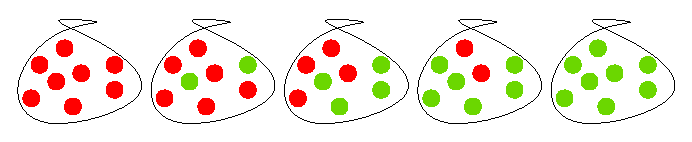
\includegraphics[width=0.7\textwidth]{images/candies.eps}
\end{center}
with the following probability distribution\begin{itemize}
    \item $\Prob(h_1)=10\%$, $h_1$ is the bag with $100\%$ cherry candies.
    \item $\Prob(h_2)=20\%$, $h_2$ is the bag with $75\%$ cherry candies.
    \item $\Prob(h_3)=40\%$, $h_3$ is the bag with $50\%$ cherry candies.
    \item $\Prob(h_4)=20\%$, $h_4$ is the bag with $25\%$ cherry candies.
    \item $\Prob(h_5)=10\%$, $h_5$ is the bag with $0\%$ cherry candies.
\end{itemize}
We choose a random bag and we want to estimate what kind of bag is it, and what is the probability of extracting a candy of a specific flavor next. We define $\Prob(c)$ the probability of extract a cherry candy, $\Prob(l)$ the probability of extract a lime candy,  the likelihood probability for lime candy is\begin{align*}
    &\Prob(l,h_1)=0\\
    &\Prob(l,h_2)=0.25\\
    &\Prob(l,h_3)=0.5\\
    &\Prob(l,h_4)=0.75\\
    &\Prob(l,h_5)=1
\end{align*}
the probability of extracting a lime candy without having any data is\begin{equation}
    \sum_{i=1}^5\Prob(l|h_i)\Prob(h_i)=\frac{1}{2}.
\end{equation}
We consider now the following data set $D_1=\{l\}=\{\text{first candy is lime}\}$, for the Bayes rule we know that\begin{equation}
    \Prob(h_i|D_1)=\frac{\Prob(D_1|h_i)\Prob(h_i)}{\Prob(D_1)}
\end{equation}
we set $\Prob(D_1)^{-1}=\alpha$, that is a normalization factor, we have that\begin{align*}
    &\Prob(h_1|D_1)=\alpha\Prob(D_1|h_1)\Prob(h_1)=\alpha(0\cdot 0.1)=0\\
    &\Prob(h_2|D_1)=\alpha\Prob(D_1|h_2)\Prob(h_2)=\alpha(0.25\cdot 0.2)=\alpha0.05=0.1\\
    &\vdots 
\end{align*}
the final distribution is
\begin{center}
    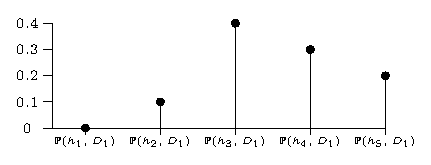
\includegraphics[width=0.7\textwidth]{images/distr_candy.eps}
\end{center}
So, let's extract another candy, the dataset is now $D_2=\{l,l\}$, the distribution become\begin{equation}
    \Prob(H|D_2) = \begin{pmatrix}
        0&0.038&0.308&0.346&0.308
    \end{pmatrix}
\end{equation}
if $D_3=\{l,l,l\}$ the distribution become\begin{equation}
    \Prob(H|D_3) = \begin{pmatrix}
        0&0.013&0.211&0.355&0.421
    \end{pmatrix}
\end{equation}
we want to calculate the probability of extracting another lime candy\begin{align*}
    &\Prob(l|D_3)=\sum_{i=1}^5\Prob(l|h_i)\Prob(h_i|D_3)\\
    &= 0 \cdot 0 + 0.25 \cdot 0.013 + 0.5 \cdot 0.211 + 0.75 \cdot 0.355 + 1 \cdot 0.421\\
    &=0.8
\end{align*}
if we use $h_{MAP}$, the answer will be $h_5\implies \Prob(l|h_5)=1$, which is not correct.\bigskip

The graph shown in figure \ref{img:candy_graph} shows how the probability that the solution is a given hypothesis $h_i$ change with the number of lime candy extracted (with 0 cherry candy extracted).

\begin{figure}[h!]
    \centering
    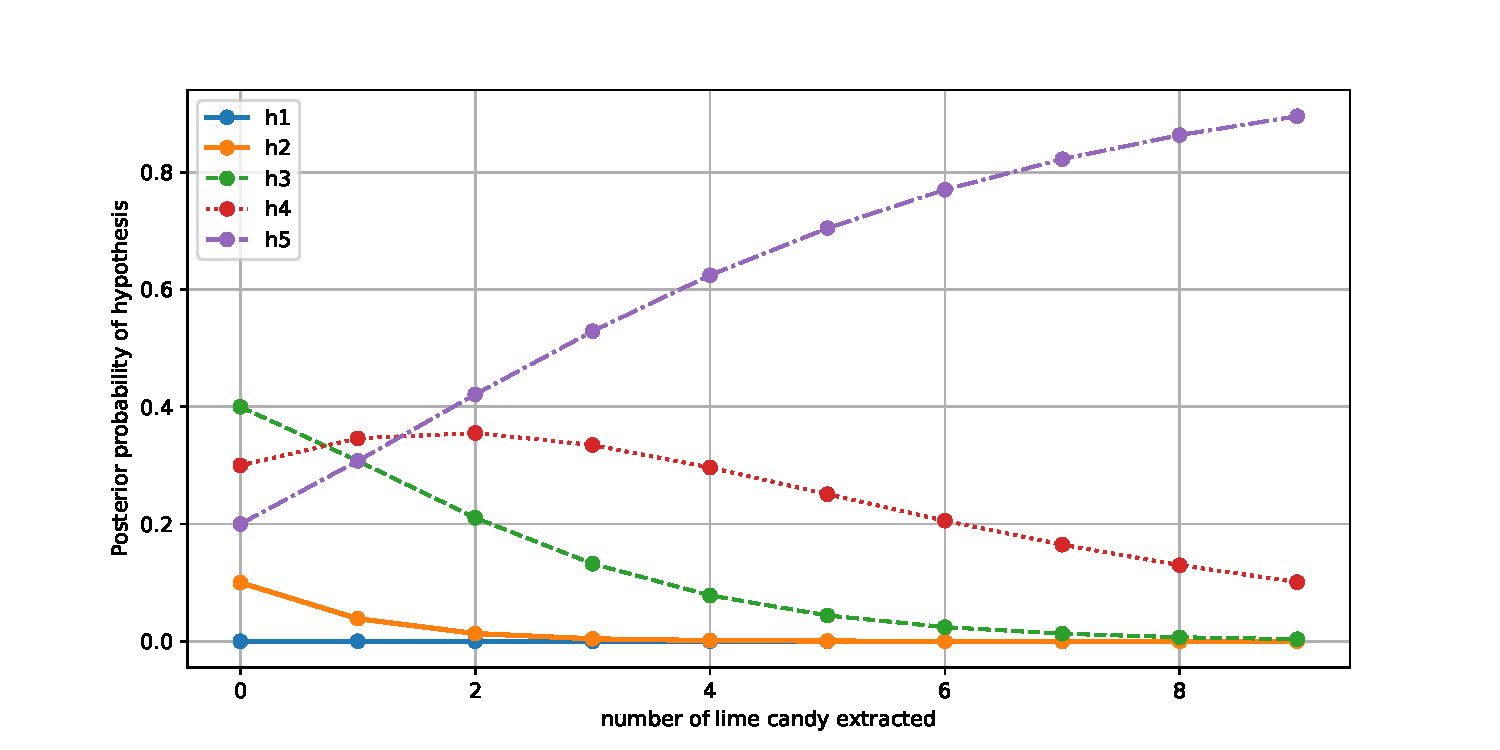
\includegraphics[width=0.8\textwidth]{images/candy_graph.pdf}
    \caption{probability of each hypothesis}
    \label{img:candy_graph}
\end{figure}
\noindent
Let's now consider an example with a continuous hypothesis space\begin{align}
    &h_\theta\in H, \ \theta\in[0,1]\\
    &\Prob(c|h_\theta)=\theta\\
    &\Prob(l|h_\theta)=1-\theta
\end{align}
the \textbf{maximum likelihood hypothesis} is\begin{equation}
    h_{ML}=\arg\max_{\theta\in[0,1]}\Prob(D|h_\theta)
\end{equation}
where with $\Prob(D|h_\theta)$ we denote the \redText{ TODO }
for the properties of the arg max function, this value is equal to
\begin{equation}
    h_{ML}=\arg\max_{\theta\in[0,1]}L(D,h_\theta)
\end{equation}
if \begin{equation}
    L(D,h_\theta)=\log\Prob(D|h_\theta)
\end{equation}
we have that\begin{equation}
    \Prob(D|h_{\theta})=\prod_{j=1}^{|D|}\Prob(d_j|h_\theta)=\theta^c(1-\theta)^l
\end{equation}
where\begin{align*}
    &d_j\in D\\
    &l = \text{ number of lime candies in }D\\
    &c = \text{ number of cherry candies in }D.
\end{align*}
So\begin{equation}
    L(D,h_\theta)=\log(\theta^c(1-\theta)^l)=c\log\theta+l\log(1-\theta)
\end{equation}
to find the value of $\theta$ that maximize $\Prob(D|h_\theta)$ we can find the maximum value of $ L(D,h_\theta)$ by considering the derivative:\begin{align*}
    &\frac{dL}{d\theta}=\frac{c}{\theta}-\frac{l}{1-\theta}
\end{align*}
we find the maximum value by imposing $\frac{dL}{d\theta}=0$\begin{equation}
    \frac{c}{\theta}-\frac{l}{1-\theta}=0\iff \theta=\frac{c}{c+l}=\frac{c}{|D|}=\theta^*
\end{equation}
so $h_{\theta^*}$ is the maximum likelihood hypothesis, this is trivial.\bigskip

In the general case, we have a dataset $D=\bigcup_i d_i$, we assume a probability distribution $\Prob(d_i|h)$ and we find the Maximum likelihood estimation\begin{equation}
    h_{ML}=\arg\max_{h\in H}\log\Prob(D|h)
\end{equation}
this can't be solved analytically for some distributions.
\subsection{Naive Bayes Classifier}
\begin{itemize}
    \item with a discrete problem we can apply the Bayes Optimal Classifier, provides the best result but is not practical if the hypothesis space is large.
    \item with a continuous model we consider the maximum likelihood estimation when analytical solutions are available.
\end{itemize}
What happens if we can't apply the previous methods? We use the assumption of conditional independence.\begin{definition}
    $X$ is conditionally independent of $Y$ given $Z$ if\begin{equation}
        \Prob(X, Y|Z)= \Prob(X|Y,Z)\Prob(Y|Z)=\Prob(X|Z)\Prob(Y|Z).
    \end{equation}
\end{definition}
This assumption in practice is usually not true, so the solution will be approximated.
Let's consider a target function $$f:X\rightarrow V $$ where each instance $x\in X$ is described by different attributes $$x=(a_1,a_2\dots, a_n)$$
we compute\begin{equation}
    \arg\max_{v\in V}\Prob(v|x,D)
\end{equation}
we express $x$ in terms of the attributes\begin{align}
    &\arg\max_{v\in V}\Prob(v|a_1,a_2\dots, a_n,D)\\
    &=\arg\max_{v\in V}\Prob(a_1,a_2\dots, a_n|v,D)\Prob(v|D)
\end{align}
then we assume that the attributes are conditionally independent\begin{equation}
    \Prob(a_1,a_2\dots, a_n|v,D)=\prod_{i=1}^{n} \Prob(a_i|v,D)
\end{equation}
so the \textbf{Naive Bayes Classifier} is the learned function:\begin{equation}
    v_{NB}(x)=v_{NB}(a_1\dots, a_n)=\arg\max_{v\in V}\Prob(v|D)\prod_{i=1}^{n} \Prob(a_i|v,D)
\end{equation}
Clearly the assumption that the attributes are independent ins wrong, consider the tennis example \ref{tab:tennis_data_big}, if the outlook is $Rain$, the probability that the temperature is $hot$ is lower than the probability that is $cool$.\bigskip

The algorithm \ref{alg:naive_bayes} show the procedure of the naive Bayes classifier estimation in the case of a classification problem.\bigskip

\begin{algorithm}
    \caption{Naive Bayes Classifier}\label{alg:naive_bayes}
    \begin{algorithmic}
    \Require a dataset $D$, target function $f:X\rightarrow V$,$X=A_1\times \dots \times A_n$, a new instance $x=(a_1\dots,a_n)$
    \For{each $v_j\in V$}
    \State $\hat \Prob(v_j|D)\longleftarrow$\texttt{estimate}$(\Prob(v_j|D))$
    \For{each attribute $A_k$}
    \For{each $a_i^k\in A_k$}
    \State $\hat \Prob(a_i^k|v_j,D)\longleftarrow$\texttt{estimate}$(\Prob(a_i^k|v_j,D))$
    \EndFor
    \EndFor
    \EndFor
    \end{algorithmic}
\end{algorithm}

After the probability $\hat\Prob$ are estimated, the new instance is classified\begin{equation}
    v_{NB}=\arg\max_{v\in V}\hat\Prob(v|D)\prod_{i=1}^{n}\hat\Prob(a_i^k|v,D).
\end{equation}
How the probabilities are estimated? For $v_j\in V$ is considered the set the samples with $v_j$ as label\begin{equation}
    D_{v_j}=\{(x,v)\in D \ : \ v=v_j\}
\end{equation}
then the estimated probability is \begin{equation}
    \hat\Prob(v_j|D)=\frac{|D_{v_j}|}{|D|}
\end{equation}
given $a_i^k\in A_k$, for $\hat \Prob(a_i|v_j,D)$, we consider the set of all samples such that, their $A_k$ attribute have $a_i^k$ as a value\begin{align}
    &D_{a_i^k}=\{(a^1,a^2\dots a^k \dots , a^n,v)\in D \ : \ a^k=a^k_i\}\\
    &\hat \Prob(a_i^k|v_j,D)=\frac{|D_{a_i^k}|}{|D_{v_j|}}
\end{align}
usually, in the estimation are included two real number $p,m$ such that\begin{equation}
    \hat \Prob(a_i^k|v_j,D)=\frac{|D_{a_i^k}|+mp}{|D_{v_j|}+m}
\end{equation}
where\begin{itemize}
    \item $p$ is a prior estimation for $\Prob(a_i^k|v_j,D)$
    \item $m$ is a weight given to that prior estimation.
\end{itemize}
Even if the conditional independence assumption is often violated the naive Bayes classifier works surprisingly well, to make that the method works correctly, we don't need that the posteriori estimation $\hat\Prob(v_j|x,D)$ to be correct, but we need that\begin{equation}
    \arg\max_{v\in V}\hat\Prob(v|D)\prod_{i=1}^{n}\hat\Prob(a_i^k|v,D)=\arg\max_{v\in V}\Prob(v|D)\Prob(a_1\dots, a_n|v,D).
\end{equation}
\subsection{Text Classification}
In this section we explain how to model a simple document classifier using the naive Bayes approach, the target function, given a document, returns the the class of that document (e.g. Scientific Article, Recipe, Poem, ecc...). This classifier have multiple application, in example:\begin{itemize}
    \item Spam classification for e-mail
    \item Sentiment analysis
\end{itemize}
Let $f$ to be the target function, $C=\{c_1,\dots c_k\}$ the set of the classes, and $Docs$ the set of documents. $D=\bigcup_{i=1}^n\{(doc_i,c_i)\}$ is the dataset. We want to compute\begin{equation}
    c_{NB}(doc)=\arg\max_{c_j\in C}\Prob(c_j|D)\Prob(doc|c_j,D).
\end{equation}
We want to express each document $doc$ as a ordered list of words, we define a vocabulary\begin{equation}
    V=\{w_1,w_2\dots w_n\}
\end{equation}
that contains all possible words $w_i$ that can appear in any document. Any document $doc_i\in Docs$ have a length (number of words) denoted $m_i$\begin{equation}
    doc_i=w_1w_2\dots w_{m_i}
\end{equation}
The probability that a document $doc_i$ is in class $c_j\in C$ given $D$ is\begin{equation}
    \Prob(doc_i|c_j,D)=\prod_{k=1}^{m_i}\Prob(p_k=w_k|c_j,D)
\end{equation}
where $\Prob(p_k=w_k|c_j|D)$ is the probability that, in a document $doc_i$ of class $c_j$, the word $p_k$ at position $k$ is $w_k$. We assume that the order of the words does not affect the probability\begin{equation}
    \forall,k,k' \ \ \ \Prob(p_k=w_k|c_j,D)=\Prob(p_{k'}=w_{k'}|c_j,D)
\end{equation}
so we consider only \begin{equation}
    \Prob(w_k|c_j,D)=\text{ probability that $w_k$ occurs in a document of class $c_j$ given $D$}.
\end{equation}
Each document can be represented as a $n$-dimensional vector, where the coordinate $i$ is equal to $k$ if in the document there are $k$ words $w_i\in V$. This representation looses the information about the order of the words. In this context, we denote a vector \begin{align}
    &\mathbf d = (d_1,d_2\dots d_n)\\ &d_i = \text{ number of times words $w_i$ appear in $\mathbf d$}
\end{align}
we recall that $n=|V|$ is the number of distinct words in the vocabulary, the probability of classifying $\mathbf d$ as $c_j\in C$ given $D$ is\begin{equation}
    \Prob(\mathbf d|c_j,D)=\frac{n!}{d_1!\dots d_n!}\prod_{i=1}^{n}\Prob(w_i|c_j,D)^{d_i}
\end{equation}
we recall that $\Prob(w_i|c_j,D)$ is the probability of observing the word $w_i$ given that the document $\mathbf d$ belongs to the class $c_j$.  This probability is estimated with the maximum likelihood value:\begin{equation}
    \hat\Prob(\mathbf d|c_j,D)=\frac{\displaystyle  
    \sum_{\mathbf d \in D}tf_{i,j}+\alpha
    }{\displaystyle  
    \sum_{\mathbf d \in D}tf_{j}+\alpha n
    }
\end{equation}
where\begin{itemize}
    \item $tf_{i,j}$ is the all-term frequency that $w_i$ occurs in the document $\mathbf d$ given that $\mathbf d$ is of class $c_j$ within the document dataset $D$.
    \item $tf_{j}$ is the total number of words in all document of $D$ that belongs to the class $c_j$.
    \item $\alpha$ is a smoothing parameter.
\end{itemize}
The algorithm \ref{alg:text_classifier} describes the methods that estimate the probabilities to classify new documents.\bigskip

\begin{algorithm}
    \caption{Text Classifier}\label{alg:text_classifier}
    \begin{algorithmic}
    \Require a dataset of documents $D$, a set of classes $C$
    \State $V\longleftarrow$ all distinct words in $D$
    \For{each $c_j\in C$}
    \State $docs_j\longleftarrow$ subset of $D$ of document of class $c_j$
    \State $t_j\longleftarrow |docs_j|$
    \State $\hat\Prob(c_j)\longleftarrow \frac{t_j}{|D|}$
    \State $TF_j\longleftarrow$ total number of words in $docs_j$ (counting duplicates)
    \For{$w_i\in V$}
    \State $TF_{i,j}\longleftarrow$ total number of times that $w_i$ occurs in $docs_j$
    \State $\hat\Prob(w_i|c_j)\longleftarrow \frac{TF_{i,j}+1}{TF_j+|V|}$
    \EndFor
    \EndFor
    \end{algorithmic}
\end{algorithm}

After we got the probabilities $\hat\Prob$, we classify a new document $doc=w_1\dots w_{m}$ as follows\begin{equation}
    v_{NB}(doc)=\arg\max_{c_j\in C}\hat\Prob(c_j)\prod_{i=1}^{m}\hat\Prob(w_i|c_j)
\end{equation}
\section{Probabilistic Generative Models}
\subsection{Parametrized Hypothesis Space}
Given a target function
$$ f:X\rightarrow C $$
we have a parametrized hypothesis space if, the set of all possible solutions $H$, contains functions of the type
\begin{equation}
    y(x,\btheta)
\end{equation}
where $x\in X$ and $\btheta$ is the parameters of the function, an example is\begin{equation}
    y(x,\mathbf w)=y(x,(w_1,w_2,w_3,w_4))=\sum_{i=1}^4x^iw_i
\end{equation}
in this kinds of problem, the search of a solution, is the determination of the parameters $\btheta$. If the we have a high number of parameters, the model will be more powerful and the training will be more expensive (in computational terms).

A model could also be hyperparametrized, if the set of possible solution is parameterized by some fixed values that can't change during the training. An example of hyper parameter could be the grade of the polynomials functions in the hypothesis space $H$.
\begin{align*}
    &H=\left\{\sum_{i=1}^nw_ix^i\right\}\\
    &n\text{ is an hyperparameter}\\
    &w_1,\dots w_n\text{ are the parameters}
\end{align*}
Let's consider a classification problem, the function to learn is\begin{equation}
    f:X\rightarrow\{c_1,c_2\dots c_K\}
\end{equation}
where the input space is continuous: $X\subseteq\R^d$. We need to evaluate the probability that a given point is in a given class\begin{equation}
    \Prob(c_k|c,D) \ \ \ x\notin D 
\end{equation}
since the dataset is fixed in this context, we can write directly \begin{equation}
    \Prob(c_k|c) \ \ \ x\notin D 
\end{equation}
is implicit that the probability depends on the dataset. The \textit{main assumption} of this section is that there is a \textbf{Gaussian Distribution} over $x$, for each class $c_k$\begin{equation}
    \Prob(x|c_k)=\mathcal N(x,\mu_k,\Sigma_k)
\end{equation}
where $\mu_k$ is the mean vector and $\Sigma_k$ is the covariance matrix. To emphasize and reiterate that certain quantities are vectors, bold letters will be used in the notation.
\begin{equation}
    \Prob(\mathbf x|c_k)=\mathcal N(\mathbf  x,\bmu_k,\Sigma_k)
\end{equation}
\subsection{Models for 2 Classes}
Let's consider the case with two classes
$$ 
f:X\rightarrow\{c_1,c_2\}
$$
In this case, assuming that the distributions are gaussian, we have that\begin{align}
    &\Prob(\mathbf x|c_1)=\mathcal N(\mathbf x,\bmu_1,\Sigma_1)\\
    &\Prob(\mathbf x|c_2)=\mathcal N(\mathbf x,\bmu_2,\Sigma_2)
\end{align}
we recall that\begin{align}
    &X\subset \R^d\\ 
    &\bmu_i,\mathbf x\in\R^d\\
    &\Sigma_i\in Mat(d\times d)
\end{align}
we also have\begin{equation}
    \Prob(c_1)=p,  \ \ \ \ \Prob(c_2)=1-p
\end{equation}
now, we have to estimate the parameters $\bmu_1,\Sigma_2,\bmu_1,\Sigma_2,p$ to use $\Prob(\mathbf x|c_i)$ and make predictions on samples that are not in the dataset, since for the Bayes theorem:\begin{align}
    &\Prob(c_1|\mathbf x)=\frac{\Prob(\mathbf x|c_1)\Prob(c_1)}{\Prob(\mathbf x)}\\
    &\Prob(c_2|\mathbf x)=\frac{\Prob(\mathbf x|c_2)\Prob(c_2)}{\Prob(\mathbf x)}
\end{align}
we get (for $i=1,2$):\begin{align}
    &\Prob(c_i|\mathbf x)=\frac{\Prob(\mathbf x|c_i)\Prob(c_i)}{\Prob(\mathbf x)}=\\
    &\frac{\Prob(\mathbf x|c_i)\Prob(c_i)}{\Prob(\mathbf x|c_1)\Prob(c_1)+\Prob(\mathbf x|c_2)\Prob(c_2)}
\end{align}
setting
\begin{equation}
    a(\mathbf x)=\ln\left(\frac{\Prob(\mathbf x|c_1)\Prob(c_1)}{\Prob(\mathbf x|c_2)\Prob(c_2)}\right)
\end{equation}
we get\begin{align}
    &\Prob(c_i|\mathbf x)=\frac{\Prob(\mathbf x|c_i)\Prob(c_i)}{\Prob(\mathbf x|c_1)\Prob(c_1)+\Prob(\mathbf x|c_2)\Prob(c_2)}=\\
    &\frac{1}{1+\exp(-a(\mathbf x))}=\sigma(a(\mathbf x))
\end{align}
we call  $\sigma$ the \textbf{sigmoid function}. This function ''squeeze'' the values from $\R$ to $[0,1]$. By the assumption about the distribution, we know that\begin{equation}
    a(\mathbf x)=\ln\left(\frac{\Prob(\mathbf x|c_1)\Prob(c_1)}{\Prob(\mathbf x|c_2)\Prob(c_2)}\right)=
\ln\left(\frac{\mathcal N(\mathbf x,\bmu_1,\Sigma_1)p}{\mathcal N(\mathbf x,\bmu_2,\Sigma_2)(1-p)}\right)
\end{equation}
We do an ulterior assumption, the covariance matrices are equals: $\Sigma_1=\Sigma_2$.
\begin{equation}
    a(\mathbf x)=
\ln\left(\frac{\mathcal N(\mathbf x,\bmu_1,\Sigma)p}{\mathcal N(\mathbf x,\bmu_2,\Sigma)(1-p)}\right)
\end{equation}
\begin{figure}[h!]
    \centering
    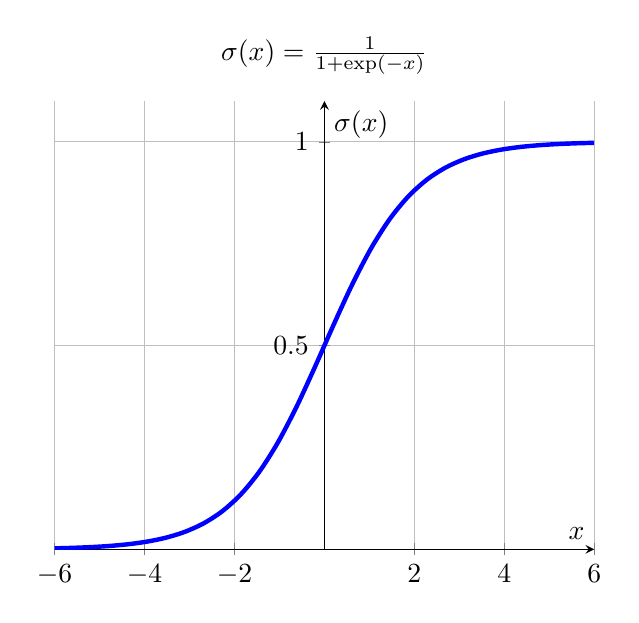
\begin{tikzpicture}[
        % Definisci la funzione sigmoide per poterla riutilizzare facilmente
        declare function={sigmoid(\x)=1/(1+exp(-\x));}
    ]
    \begin{axis}[
        % Impostazioni dell'asse
        title={$\sigma(x) = \frac{1}{1 + \exp(-x)}$},
        xlabel={$x$},
        ylabel={$\sigma(x)$},
        axis lines=middle, % Assi centrati all'origine
        xmin=-6, xmax=6, % Range sull'asse x
        ymin=0, ymax=1.1, % Range sull'asse y (un po' sopra 1 per chiarezza)
        xtick={-6,-4,-2,0,2,4,6}, % Tick specifici per x
        ytick={0, 0.5, 1}, % Tick specifici per y
        grid=major, % Aggiunge una griglia per riferimento
        domain=-6:6, % Dominio di campionamento della funzione
        samples=30, % Aumenta i campioni per una curva più liscia
    ]
    \addplot[
        blue, 
        ultra thick, % Spessore della linea
        smooth % Rende la curva più smussata (anche se con 100 campioni è già liscia)
    ] {sigmoid(x)};
    \end{axis}
    \end{tikzpicture}
    \caption{Sigmoid function curve}
\end{figure}
At this point, we know that
\begin{equation}
    \Prob(c_i|\mathbf x)=\sigma(a(\mathbf x))
\end{equation}
so, given the parameters $\bmu_1,\bmu_2,p,\Sigma$, we can make prediction by the following decision rule:\begin{itemize}
    \item Given $\mathbf x\notin D$
    \item if $\Prob(c_1|\mathbf x)>0.5$ the point $\mathbf x$ is in class $c_1$
    \item else, if $\Prob(c_1|\mathbf x)\le0.5$ the point $\mathbf x$ is in class $c_2$
\end{itemize}
The parameters can be found with the maximum likelihood function, we have to introduce some notation to simplify the understanding process, the dataset is denoted:\begin{equation}
D=\{(\mathbf x_n,t_n)_{n=1}^N\}
\end{equation}
where $t_n=1$ if $\mathbf x_n$ is in class $c_1$, else $t_n=0$. This encoding is useful to write the likelihood function. We denote $\mathbf t=(t_n)_{n=1}^N$ the binary vector of the dataset's labels. The likelihood function is the probability that, given the parameters, the labels $\mathbf t$ are correct predictions:
\begin{equation}
    \Prob(\mathbf t|p,\bmu_1,\bmu_2,\Sigma,D)=\prod_{n=1}^{N}
    \left(
    p\mathcal N(\mathbf x_n,\bmu_1,\Sigma)
    \right)^{t_n}
    \left(
    (1-p)\mathcal N(\mathbf x_n,\bmu_2,\Sigma)
    \right)^{(1-t_n)}
\end{equation}
The ML solution is given by the parameters that maximize that function (we use the natural logarithm):\begin{equation}
    \hat p,\hat\bmu_1,\hat\bmu_2,\hat\Sigma=\arg\max_{p,\bmu_1,\bmu_2,\Sigma}\ln\Prob(\mathbf t|p,\bmu_1,\bmu_2,\Sigma,D)
\end{equation}
In this context the function is analytical and we have a closed form solution, the parameters that maximize that function are\begin{align}
    &\hat p=\frac{N_1}{N}, \ \ \ \text{ where } N_1=|\{(\mathbf x,t)\in D \ : \ t=1\}|\\
    &\hat\bmu_1=\frac{1}{N_1}\sum_{n=1}^Nt_n\mathbf x_n\\
    &\hat\bmu_2=\frac{1}{N_2}\sum_{n=1}^N(1-t_n)\mathbf x_n\\
\end{align}
The matrix $\Sigma$ needs the definition of the two matrices\begin{align}
    &S_1=\frac{1}{N_1}\sum_{(\mathbf x_n,t_n)\in D \ : \ t_n=1}(\mathbf x_n-\hat \bmu_1)(\mathbf x_n-\hat \bmu_1)^T\\
    &S_2=\frac{1}{N_1}\sum_{(\mathbf x_n,t_n)\in D \ : \ t_n=0}(\mathbf x_n-\hat \bmu_2)(\mathbf x_n-\hat \bmu_2)^T
\end{align}
then\begin{align}
    &\hat \Sigma = \frac{N_1}{N}S_1+\frac{N_2}{N}S_2
\end{align}
note that the with $(\mathbf x_n-\hat \bmu_i)(\mathbf x_n-\hat \bmu_i)^T$ is denoted the matrix multiplication between a $d\times 1$ matrix and a $1\times d$ matrix.\bigskip

The function $a(\mathbf x)$ includes non linear terms, since it includes the Gaussian distribution, apparently, is a non linear function. The following statement is crucial.
\begin{theorem}
    the function $a(\mathbf x)$ is linear in $\mathbf x$.
\end{theorem}
\textit{Proof}: We have to show that, there exists $\mathbf w\in \R^d$ and $w_0\in \R$ such that\begin{equation}
a(\mathbf x)=
\ln\left(\frac{\mathcal N(\mathbf x,\bmu_1,\Sigma)p}{\mathcal N(\mathbf x,\bmu_2,\Sigma)(1-p)}\right)=\mathbf w^T\mathbf x+w_0
\end{equation}
For the logarithms properties we have:\begin{align}
    &a(\mathbf x)=
\ln\left(\frac{\mathcal N(\mathbf x,\bmu_1,\Sigma)p}{\mathcal N(\mathbf x,\bmu_2,\Sigma)(1-p)}\right)=\\
&\ln\left(\frac{\mathcal N(\mathbf x,\bmu_1,\Sigma)}{\mathcal N(\mathbf x,\bmu_2,\Sigma)}\right)-\ln\left(\frac{p}{1-p}\right)
\end{align}
we expand the Gaussian distribution form:\begin{align}
    &\ln\left(\frac{ \frac{1}{\sqrt{(2\pi)^d}\det\Sigma}\exp(-\frac{1}{2}(\mathbf x-\bmu_1)^T\Sigma^{-1}(\mathbf x-\bmu_1))}{
        \frac{1}{\sqrt{(2\pi)^d}\det\Sigma}\exp(-\frac{1}{2}(\mathbf x-\bmu_2)^T\Sigma^{-1}(\mathbf x-\bmu_2))
    }\right)-\ln\left(\frac{p}{1-p}\right)
\end{align}
since the covariance matrices are equals, the term $\frac{1}{\sqrt{(2\pi)^d}\det\Sigma}$ get cancelled\begin{align}
    &\ln\left(\frac{\exp(-\frac{1}{2}(\mathbf x-\bmu_1)^T\Sigma^{-1}(\mathbf x-\bmu_1))}{
        \exp(-\frac{1}{2}(\mathbf x-\bmu_2)^T\Sigma^{-1}(\mathbf x-\bmu_2))
    }\right)-\ln\left(\frac{p}{1-p}\right)
\end{align}
Due to the properties of exponentials and logarithms, the logarithm of a ratio is the difference of the logarithms:\begin{align}
    &-\frac{1}{2}(\mathbf x-\bmu_1)^T\Sigma^{-1}(\mathbf x-\bmu_1)-
    (-\frac{1}{2}(\mathbf x-\bmu_2)^T\Sigma^{-1}(\mathbf x-\bmu_2))
    -
    \ln\left(\frac{p}{1-p}\right)
\end{align}
we multiply by $-2$ and we get\begin{align}
    &(\mathbf x-\bmu_1)^T\Sigma^{-1}(\mathbf x-\bmu_1)-
    (\mathbf x-\bmu_2)^T\Sigma^{-1}(\mathbf x-\bmu_2)
    +
    2\ln\left(\frac{p}{1-p}\right)
\end{align}
$(\mathbf x-\bmu_i)^T\Sigma^{-1}(\mathbf x-\bmu_i)$ are quadratic forms and can be expanded (remember that $\Sigma$ is symmetric):
\begin{align}
    &\mathbf x^T\Sigma^{-1}\mathbf x-2\bmu_1^T\Sigma^{-1}\mathbf x+\bmu_1^T\Sigma^{-1}\bmu_1
    -
    \mathbf x^T\Sigma^{-1}\mathbf x-2\bmu_2^T\Sigma^{-1}\mathbf x+\bmu_2^T\Sigma^{-1}\bmu_2
    +
    2\ln\left(\frac{p}{1-p}\right)=\\
    &-2\bmu_1^T\Sigma^{-1}\mathbf x+\bmu_1^T\Sigma^{-1}\bmu_1
    -2\bmu_2^T\Sigma^{-1}\mathbf x+\bmu_2^T\Sigma^{-1}\bmu_2
    +
    2\ln\left(\frac{p}{1-p}\right)
\end{align}
reordering we get:\begin{equation}
    2(\bmu_2-\bmu_1)^T\Sigma^{-1}\mathbf x+(\bmu_1^T\Sigma^{-1}\bmu_1-\bmu_2^T\Sigma^{-1}\bmu_2)+
    2\ln\left(\frac{p}{1-p}\right)
\end{equation}
we call $r$ the constant $(\bmu_1^T\Sigma^{-1}\bmu_1-\bmu_2^T\Sigma^{-1}\bmu_2)+
    2\ln\left(\frac{p}{1-p}\right)$
    \begin{equation}
    2(\bmu_2-\bmu_1)^T\Sigma^{-1}\mathbf x+r
\end{equation}
remember that we have to re-multiply by $-\frac{1}{2}$:
\begin{equation}
    -(\bmu_2-\bmu_1)^T\Sigma^{-1}\mathbf x-\frac{1}{2}r
\end{equation}
we define\begin{align}
    &\mathbf w=(-(\bmu_2-\bmu_1)^T\Sigma^{-1})^T\\ 
    &w_0=-\frac{1}{2}r=-\frac{1}{2} (\bmu_1^T\Sigma^{-1}\bmu_1-\bmu_2^T\Sigma^{-1}\bmu_2)+
    \ln\left(\frac{p}{1-p}\right)
\end{align}
in the end we have:\begin{equation}
    a(\mathbf x)=\mathbf w^T\mathbf x+w_0
\end{equation}
\hfill$\blacksquare$
\subsection{Models for $k$ Classes}
In this case we have a target function\begin{equation}
    f:X\rightarrow\{c_1,c_2\dots,c_K\}
\end{equation}
we encode the dataset as follows\begin{equation}
    D=\{(\mathbf x_n,\mathbf t_n)\}_{n=1}^N
\end{equation}
where $\mathbf t_n=(t_{n1},\dots t_{nK})$ and $t_{nk}=1\iff$ the $n$-th sample is labeled as class $c_k$.\begin{equation}
     t_{nk}=1\iff f(\mathbf x_n)=c_k
\end{equation}
we estimate $\Prob(c_k|\mathbf x)$ as follows:\begin{equation}
    \Prob(c_k|\mathbf x)=\frac{\Prob(\mathbf x|c_k)\Prob(c_k)}{\sum_{j=1}^K\Prob(\mathbf x|c_j)\Prob(c_j)}=\frac{\exp(a_k)}{\sum_{j=1}^K\exp(a_j)}
\end{equation}
where\begin{equation}
    a_j=\ln\left(\Prob(\mathbf x|c_j)\Prob(c_j)\right)
\end{equation}
we assume that $\Prob(\mathbf x|c_k)$ is Gaussian\begin{equation}
    \Prob(\mathbf x|c_k)=\mathcal N(\mathbf x,\bmu_k,\Sigma)
\end{equation}
and for each class $c_k$, we have that\begin{equation}
    \Prob(c_k)=p_k 
\end{equation}
where \begin{equation}
    \sum_{j=1}^Kp_j=1
\end{equation}
so the parameters of the model are\begin{align}
    &p_1,p_2,\dots p_K\in \R\\
    &\bmu_1,\bmu_2\dots \bmu_K\in\R^d\\ 
    &\Sigma\in Mat(d\times d)
\end{align}
denoting $\mathbf t$ the set of labels in $D$\begin{equation}
    \mathbf t = \begin{pmatrix}
        \mathbf t_1 & \dots & \mathbf t_N
    \end{pmatrix}
\end{equation}
the maximum likelihood solution is given by:\begin{equation}
    \hat p_1,\dots \hat p_k,\hat \bmu_1,\dots \hat \bmu_k,\hat \Sigma=\arg\max_{p_k,\bmu_k,\Sigma}\ln\left(
    \Prob(\mathbf t|p_1,\dots p_k,\bmu_1,\dots \bmu_k,\Sigma)
    \right)
\end{equation}
the solution can be found analytically and is\begin{align}
    &\hat p_k=\frac{N_k}{N}\text{ where }N_k=|\{(\mathbf x_n,\mathbf t_n)\in D \ : \ t_{nk}=1\}|\\
    &\hat\bmu_k=\frac{1}{N_k}\sum_{n=1}^Nt_{nk}\mathbf x_n\\ 
    &S_k=\frac{1}{N_k}\sum_{n=1}^Nt_{nk}(\mathbf x_n-\hat\bmu_k)(\mathbf x_n-\hat\bmu_k)^T\\
    &\hat \Sigma = \sum_{k=1}^{K}\frac{N_k}{N}S_k
\end{align}
a new sample $\mathbf x'\notin D$ can be predicted as follows:\begin{equation}
    h^*(\mathbf x')=\arg\max_k\frac{\exp(a_k)}{\sum_j\exp(a_j)}
\end{equation}
where $a_k=\ln\left(\hat p_k\mathcal N(\mathbf x',\hat\bmu_k,\hat\Sigma)\right)$.
\subsection{Naive Bayes Assumption}
We can consider an ulterior assumption, that the features of the samples are conditional independent, given a sample $\mathbf x_n\in \R^d$:\begin{equation}
    \Prob(\mathbf x_n|c_k)=\prod_{j=1}^d\Prob(x_{nj}|c_k)
\end{equation}
in this case, for each class $c_k$, we don't have a multivariate Gaussian distribution $\mathcal N(\mathbf x_n,\bmu_k,\Sigma)$, but we have $d$ one-dimensional Gaussian distribution\begin{equation}
    \Prob(x_{nj}|c_k)=\mathcal N(x_{nj},\mu_{jk},\sigma_{jk})
\end{equation}so the parameters of the model are
\begin{equation}
    \begin{matrix}
        p_k\in\R\\ 
        \mu_{jk}\in \R\\ 
        \sigma_{jk}\in \R
    \end{matrix} \ \text{ where } \ 
    \begin{matrix}
        j=1,\dots d\\ k=1,\dots K
    \end{matrix}
\end{equation}
the maximum likelihood solution can be found analytically:\begin{align}
    &\hat p_k=\frac{N_k}{N}\\ 
    &\hat\mu_{jk}=\frac{1}{N_k}\sum_{n=1}^Nt_{nk}x_{nj}\\
    &\hat\sigma_{jk}=\sum_{n=1}^Nt_{nk}(x_{nj}-\hat\mu_{jk})^2
\end{align}
\subsubsection{About the Number of Parameters}
Given a classification problem$$f:\R^d\rightarrow\{c_1\dots c_K\}$$
what are the size (number of parameters) of the generative model? We have the probabilities$$\Prob(c_k)=p_k $$ this counts as $K-1$ parameters, since the first $K-1$ can be used to calculate $p_K$\begin{equation}
    p_K=1-\sum_{k=1}^{K-1}p_k
\end{equation}
then we have $K$ vectors $\bmu_K$, of each $k$-th Gaussian distribution, since each vector have $d$ real components, we have a total of $kd$ parameter. In the end, we have 
\section{Discriminative Models}
\redText{TODO}
\chapter{Linear Models}
\section{Classification with Linear Models}
A linear function on $\mathbf x$ is represented as follows\begin{equation}
    \mathbf w^T\mathbf x+w_0
\end{equation}
we want to use a compact notation, adding a component to the vector $\mathbf x$:\begin{align}
    &\mathbf x \in \R^d\longrightarrow \tilde{\mathbf x}\in \R^{d+1}\\
    &\mathbf x=\begin{pmatrix}
        x_1&\dots x_d
    \end{pmatrix}^T\\
    &\tilde{\mathbf x}=\begin{pmatrix}
        1&x_1&\dots x_d
    \end{pmatrix}^T\\
    &\tilde{\mathbf w}=\begin{pmatrix}
        w_0&w_1&\dots w_d
    \end{pmatrix}^T
\end{align}
so\begin{equation}
    \mathbf w^T\mathbf x +w_0=\tilde{\mathbf w}^T\tilde{\mathbf x}=w_0+w_1x_1\dots w_dx_d.
\end{equation}
In general, we have an error function $E(\mathbf w)$ that we want to minimize\begin{equation}
    \mathbf w^*=\arg\min_{\mathbf w}E(\mathbf w)
\end{equation} 
Let's consider binary classification, there are a set of samples $D=\{(\mathbf x_n,t_n)_{n=1}^N\}$ where $\mathbf x_n\in \R^d$ and $t_n\in\{-,+\}$, we say that $D$ is \textbf{linearly separable} if there exists an hyper plane $$ \{\mathbf x \  : \ \mathbf a^T\mathbf x+\mathbf b= 0\}$$ such that\begin{align}
    &t_n=+\iff \mathbf a^T\mathbf x_n+\mathbf b\le 0\\ 
    &t_n=-\iff \mathbf a^T\mathbf x_n+\mathbf b> 0
\end{align}
In $\R^2$, a data set is linearly separable if there exists a line such that all and only the $+$ samples are in one of the half space generated by the line.\bigskip

\begin{figure}[h!]
    \centering
    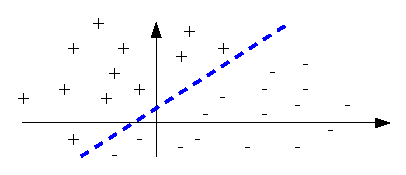
\includegraphics[width=0.5\textwidth]{images/linsep.eps}
    \caption{linearly separable data}
    \label{img:linsep}
\end{figure}

If such an hyperplane exists, can be found with a linear model by tuning $d+1$ parameters $\mathbf w, w_0$ (we consider the compact notation and we denote $\mathbf w$ the whole set of parameters) $$ \mathbf x^T\mathbf w=\begin{pmatrix}
    1&x_1 &\dots & x_n
\end{pmatrix}\begin{pmatrix}
    w_0\\w_1 \\\vdots \\ w_n
\end{pmatrix}.$$

The hyperplane that we want to find is called \textbf{linear discriminant}. 
We consider the binary notation for the samples, the target function have $K$ classes as the image, if 
$$ (\mathbf x_n,\mathbf t_n)\in D$$
then $\mathbf t_n$ is a binary vector of $K$ components, where the $i$-th coordinate of  $\mathbf t_n$ is 1 if and only if $\mathbf x_n$ is labeled with class $i$
$$ 
\mathbf t^T_n=\begin{pmatrix}
    0&0&\dots 1 & \dots & 0
\end{pmatrix}
.
$$
In the case of multiple classes, let's say $K$, we don't have a vector $\mathbf w$, but we have $K$ linear functions $\mathbf w_1\dots \mathbf w_k$, for each new sample $\mathbf x$ we calculate a prediction vector\begin{equation}
    \mathbf y(\mathbf x)=\begin{pmatrix}
        \mathbf w_1^T\mathbf x\\ \vdots \\ \mathbf w_K^T\mathbf x
    \end{pmatrix}
\end{equation}
Since we have $K$ vectors of $d$ components as parameter, we can describe all the parameters in compact notation with a matrix $W$\begin{equation}
    W=\begin{pmatrix}
        \mathbf w_1& \dots& \mathbf w_K
    \end{pmatrix}
\end{equation}
the predictions are calculated by\begin{equation}
    \mathbf y(\mathbf x)=W^T\mathbf x
\end{equation}
\subsection{Least Square Methods}
We define the $T$ matrix as the matrix where the rows are the transpose vector $\mathbf t_n$\begin{equation}
    T=\begin{pmatrix}
        \mathbf t^T_1\\ 
        \mathbf t^T_2\\ \vdots \\ 
        \mathbf t^T_N
    \end{pmatrix}\in Mat(N\times K)
\end{equation}
then, we define  the matrix $X$ as the matrix where the rows are the transpose vector $\mathbf x$ (with 1 as the first component, since we are using the compact notation).\begin{equation}
    X=\begin{pmatrix}
        \mathbf x_1^T\\ 
        \mathbf x_2^T\\ \vdots \\ 
        \mathbf x_N^T
    \end{pmatrix}=\begin{pmatrix}
        1&x_{11}&x_{12}&\dots &x_{1d}\\ 
        1&x_{21}&x_{22}&\dots &x_{2d}\\ 
        \vdots &\vdots & \vdots &\ddots & \vdots\\ 
        1&x_{N1}&x_{N2}&\dots &x_{Nd}
    \end{pmatrix}\in Mat(N\times d)
\end{equation}
let $W=\begin{pmatrix}
        \mathbf w_1& \dots& \mathbf w_K
    \end{pmatrix}$ to be the parameters of the linear model, the product $XW$ is: \begin{align}
   &XW = \begin{pmatrix}
        1&x_{11}&x_{12}&\dots &x_{1d}\\ 
        1&x_{21}&x_{22}&\dots &x_{2d}\\ 
        \vdots &\vdots & \vdots &\ddots & \vdots\\ 
        1&x_{N1}&x_{N2}&\dots &x_{Nd}
    \end{pmatrix}\begin{pmatrix}
        \mathbf w_0&\mathbf w_1&\dots & \mathbf w_K
    \end{pmatrix}=\\ \\
    &\begin{pmatrix}
        1&x_{11}&x_{12}&\dots &x_{1d}\\ 
        1&x_{21}&x_{22}&\dots &x_{2d}\\ 
        \vdots &\vdots & \vdots &\ddots & \vdots\\ 
        1&x_{N1}&x_{N2}&\dots &x_{Nd}
    \end{pmatrix}
    \begin{pmatrix}
        w_{00} & w_{01} & \dots & w_{0d}\\
        w_{10} & w_{11} & \dots & w_{1d}\\
        \vdots &\vdots & \vdots &\ddots & \vdots\\ 
        w_{K0} & w_{K1} & \dots & w_{Kd}
    \end{pmatrix}=\\  \\
    &\begin{pmatrix}
        \mathbf w^T_1\mathbf x_1 &\mathbf w^T_2\mathbf x_1 &\dots & \mathbf w^T_K\mathbf x_1\\ 
        \mathbf w^T_1\mathbf x_2 &\mathbf w^T_2\mathbf x_2 &\dots & \mathbf w^T_K\mathbf x_2\\
        \vdots &\vdots & \vdots &\ddots & \vdots\\
        \mathbf w^T_1\mathbf x_N &\mathbf w^T_2\mathbf x_N  &\dots & \mathbf w^T_K\mathbf x_N 
    \end{pmatrix} =\\ \\ &\begin{pmatrix}
        \mathbf y(\mathbf x_1)^T\\ 
        \mathbf y(\mathbf x_2)^T\\ 
        \vdots \\ 
        \mathbf y(\mathbf x_N)^T
    \end{pmatrix}
\end{align}
So $XW$ are the predictions of the model on all the samples $\mathbf x_n$, the difference\begin{equation}
    XW-T = \begin{pmatrix}
        \mathbf y(\mathbf x_1)^T-\mathbf t_1\\ 
        \mathbf y(\mathbf x_2)^T-\mathbf t_2\\ 
        \vdots \\ 
        \mathbf y(\mathbf x_N)^T-\mathbf t_N
    \end{pmatrix}
\end{equation}
measure how different the prediction of the model are respect to the label on the sample data. Based on that, given a model $W$, we can define the \textbf{sum of squares error function}:\begin{equation}
    E(W)=\frac{1}{2}Tr\left( (XW-T)^T(XW-T) \right)
\end{equation}
Where with $Tr(A)$ we denote the trace of the matrix $A$. The parameters solution is found by the following optimization problem: \begin{equation}
    W^*=\arg\min_W\frac{1}{2}Tr\left( (XW-T)^T(XW-T) \right)
\end{equation}
this problem can be solved analytically and  the closed form solution is\begin{equation}
    W^*=(X^TX)^{-1}X^TT
\end{equation}
given a new sample $\mathbf x$, the prediction is calculated as follows:\begin{equation}
    \mathbf y(\mathbf x)={W^*}^T\mathbf x = \begin{pmatrix}
        \mathbf w_1^T\mathbf x\\ 
        \mathbf w_2^T\mathbf x\\ 
        \vdots \\ 
        \mathbf w_K^T\mathbf x
    \end{pmatrix}
\end{equation}
$\mathbf x$ is labeled in class $C_k$ if\begin{equation}
    k=\arg\max_{1\le j\le K}\mathbf w_j^T\mathbf x
\end{equation}
This method is not robust to \textit{outliers}, that is sample in $D$ that are far from all the other samples, this points ''weights'' more for the linear discriminant, and the found solution will not be consistent with the dataset, as shown in figure \ref{fig:outliers}.

\begin{figure}[h!]
    \centering
    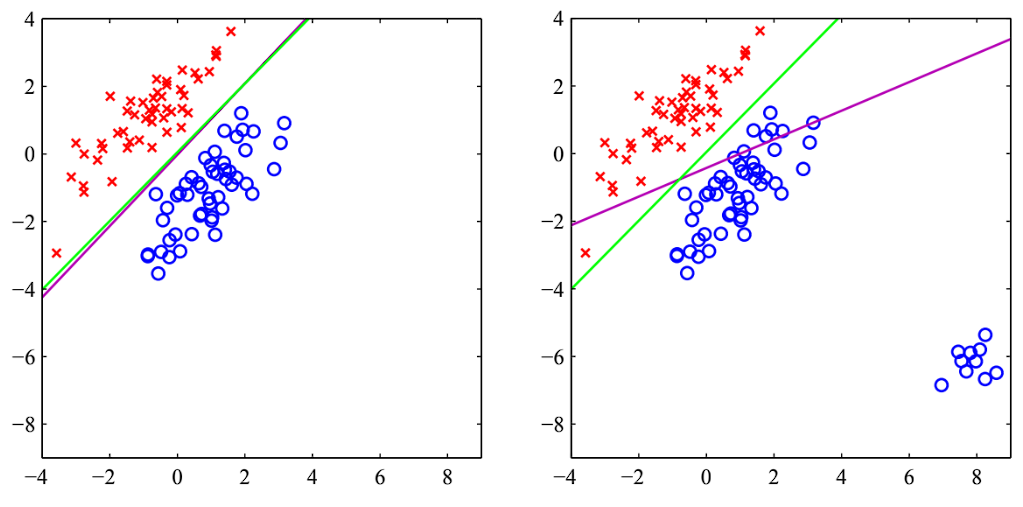
\includegraphics[width=0.5\textwidth]{images/outliers.png}
    \caption{linear discriminant without and with outliers.}
    \label{fig:outliers}
\end{figure}

\subsection{Perceptron}
A perceptron is a linear model where the output is filtered by the Heaviside step function :\begin{equation}
    o(\mathbf x)=H(\mathbf w^T\mathbf x)=\begin{cases}
        1 \text{ if }w^T\mathbf x>0\\ 
        0 \text{ if }w^T\mathbf x\le 0
    \end{cases}
\end{equation}
In this context for binary classification, the classes are denoted $-1$ and $+1$.
Given a dataset $D=\{(\mathbf x_n,t_n)_{n=1}^N\}$ with $t_n\in\{-1,+1\}$, we can consider as error function the squared error\begin{equation}
    E(\mathbf w)=\frac{1}{2}\sum_{n=1}^N(t_n-o(\mathbf x_n))=\frac{1}{2}\sum_{n=1}^N(t_n-H(\mathbf w^T\mathbf x))
\end{equation}
to find the best model $\mathbf w$ we can apply the \textit{gradient descent}, the partial derivative of $E$ respect one fo the $d+1$ parameter is\begin{align}
    &\frac{\partial E}{\partial w_i}=\\&\frac{\partial}{\partial w_i}\frac{1}{2}\sum_{n=1}^N(t_n-H(\mathbf w^T\mathbf x))=\\
    &\frac{1}{2}\sum_{n=1}^N\frac{\partial}{\partial w_i}(t_n-H(\mathbf w^T\mathbf x))
\end{align}
since the function $H$ is not differentiable, we consider the error function of the linear model without the filtering\begin{equation}
    E(\mathbf w)=\frac{1}{2}\sum_{n=1}^N(t_n-\mathbf w^T\mathbf x)
\end{equation}
in this case we can find the derivative analytically\begin{align}
    &\frac{\partial E}{\partial w_i}=\\&\frac{\partial}{\partial w_i}\frac{1}{2}\sum_{n=1}^N(t_n-\mathbf w^T\mathbf x)=\\
    &\frac{1}{2}\sum_{n=1}^N\frac{\partial}{\partial w_i}(t_n-\mathbf w^T\mathbf x)=\\
    &\sum_{n=1}^N(t_n-\mathbf w^T\mathbf x_n)\cdot (-\mathbf x_{ni})
\end{align}
so we can compute the gradient of $E$ at each point\begin{equation}
    \nabla E(\mathbf w)=\begin{pmatrix}
        \sum_{n=1}^N(t_n-\mathbf w^T\mathbf x_n)\cdot (-\mathbf x_{n1})\\ 
        \vdots \\ 
        \sum_{n=1}^N(t_n-\mathbf w^T\mathbf x_n)\cdot (-\mathbf x_{nd})
    \end{pmatrix}
\end{equation}
we denote $\mathbf x_{ni}=x_{ni}$  to emphasize that is a real number ($i$-th component of vector $\mathbf x_n$). We can consider the thresholded of the step function:\begin{equation}
    \nabla E(\mathbf w)=\begin{pmatrix}
        \sum_{n=1}^N(t_n-H(\mathbf w^T\mathbf x_n))(- x_{n1})\\ 
        \vdots \\ 
        \sum_{n=1}^N(t_n-H(\mathbf w^T\mathbf x_n))(- x_{nd})
    \end{pmatrix}
\end{equation}
$\mathbf w$ can be found by an iterative method described as follows:\begin{enumerate}
    \item initialize $\mathbf w$ with small random values 
    \item repeat the following until a termination condition:\begin{itemize}
        \item $\mathbf w\leftarrow \mathbf w-\eta\nabla E(\mathbf w)$
    \end{itemize}
    \item return $\mathbf w$
\end{enumerate}
In the step $$\mathbf w\leftarrow \mathbf w-\eta\nabla E(\mathbf w)$$
we are moving towards a direction where the error decrease.

\begin{figure}[h!]
    \centering
    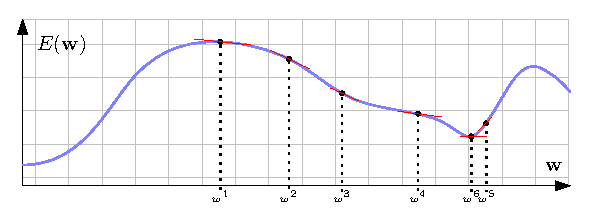
\includegraphics[width=0.7\textwidth]{images/grad_desc.eps}
    \caption{In this case $\mathbf w\in \R$, with $w^k$ is denoted the value of $\mathbf w$ at the iteration $k$.}
    \label{fig:grad}
\end{figure}

$\eta$ is a real positive value, is an hyperparameter that tells ''how strongly'' the descent follows the direction of the gradient. The more $\eta$ is small, the more the precision are high and the slow the algorithm will converge, linearly separable data and sufficient small $\eta$ ar sufficient conditions to make the algorithm converge. Since at each step we have to compute the gradient by iterating on all the samples, we can consider a variant of the methods called \textit{stochastic gradient descent} where the error function is calculated not on $D$ but on a subset $S\subset D$ extracted randomly.\begin{equation}
    \nabla E_S(\mathbf w)=\begin{pmatrix}
        \sum_{\mathbf x_n\in S}(t_n-H(\mathbf w^T\mathbf x_n))(- x_{n1})\\ 
        \vdots \\ 
        \sum_{\mathbf x_n\in S}(t_n-H(\mathbf w^T\mathbf x_n))(- x_{nd})
    \end{pmatrix}
\end{equation}
Suitable solution for the termination condition may be\begin{itemize}
    \item the error $E$ reached a sufficient small value 
    \item after a predefined number of iteration.
\end{itemize}
After we learned a model $\mathbf w^*$, a new sample $\mathbf x$ is predicted with $H({\mathbf  w^*}^T\mathbf x)$.
\subsection{Fisher's Linear Discriminant}
This method's consider a linear discriminant $\mathbf w$, and it adjust the direction of that linear function to maximize the separation of classes in the dataset, consider a dataset $D$ with points in two classes, where $N_1$ are the number of points in class $C_1$ and $N_2$ are the number of points in class $C_2$. Two vectors $\mathbf m_1,\mathbf m_2$ are calculated in the following way\begin{align}
&\mathbf m_1=\frac{1}{N_1}\sum_{\mathbf x_n\in C_1}\mathbf x_n\\ 
&\mathbf m_2=\frac{1}{N_2}\sum_{\mathbf x_n\in C_2}\mathbf x_n
\end{align}
We solve the following optimization problem:\begin{align*}
    &\max J(\mathbf w)=\mathbf w^T(\mathbf m_1-\mathbf m_2)\\ 
    \text{subject to} \ \ \ &\|\mathbf w\|=1
\end{align*}
$\mathbf m_1$ is the center of mass of the samples of class $C_1$ (analogous interpretation for $\mathbf m_2$ and $C_2$).
The value of $\mathbf w$ that maximize $\mathbf w^T(\mathbf m_1-\mathbf m_2)$ will be aligned to the vector $(\mathbf m_1-\mathbf m_2)$.\begin{center}
    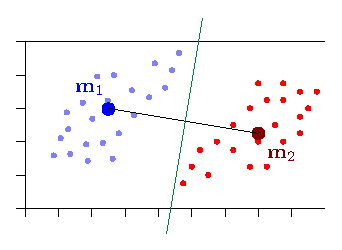
\includegraphics[width=0.4\textwidth]{images/fisher.eps}
\end{center} 
\redText{TODO}
\subsection{Support Vector Machines}
\redText{TODO}
\section{Linear Regression}
We want to use a linear model for regression, the target function is\begin{align}
    &f:X\rightarrow Y\\ 
    &X\subseteq \R^d\\ 
    &Y\subseteq \R 
\end{align}
The $d$ parameters are $\mathbf w$ and the model is\begin{equation}
    y(\mathbf x)=y(\mathbf x,\mathbf w)=\mathbf w^T\mathbf x
\end{equation}
with \begin{align*}
    &\mathbf x^T=\begin{pmatrix}
        1&x_1&\dots &x_d
    \end{pmatrix}\\ 
    &\mathbf w^T=\begin{pmatrix}
        w_0&w_1&\dots &w_d
    \end{pmatrix}
\end{align*}
\begin{center}
    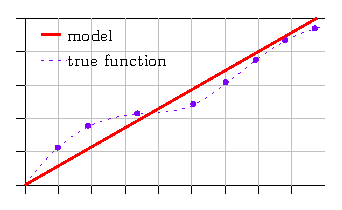
\includegraphics[width=0.4\textwidth]{images/lin_reg.eps}
\end{center} 
It is possible to consider a non linear transformation of the input $\boldsymbol{\phi}(\mathbf x)$\begin{equation}
    y(\mathbf x)=\mathbf w^T\boldsymbol{\phi}(\mathbf x)
\end{equation}
where\begin{equation}
    \boldsymbol{\phi}(\mathbf x)=\begin{pmatrix}
        \phi_0(\mathbf x)\\\phi_1(\mathbf x)\\ 
        \vdots \\ 
        \phi_M(\mathbf x)
    \end{pmatrix}
\end{equation}
An example, with $X=\R$, is $\phi_j(x)=x^j$:\begin{equation}
    y(x,\mathbf w)=\sum_{j=1}^Mw_jx^j
\end{equation}
$M$ is an hyper parameter of the machine learning problem.
\begin{center}
    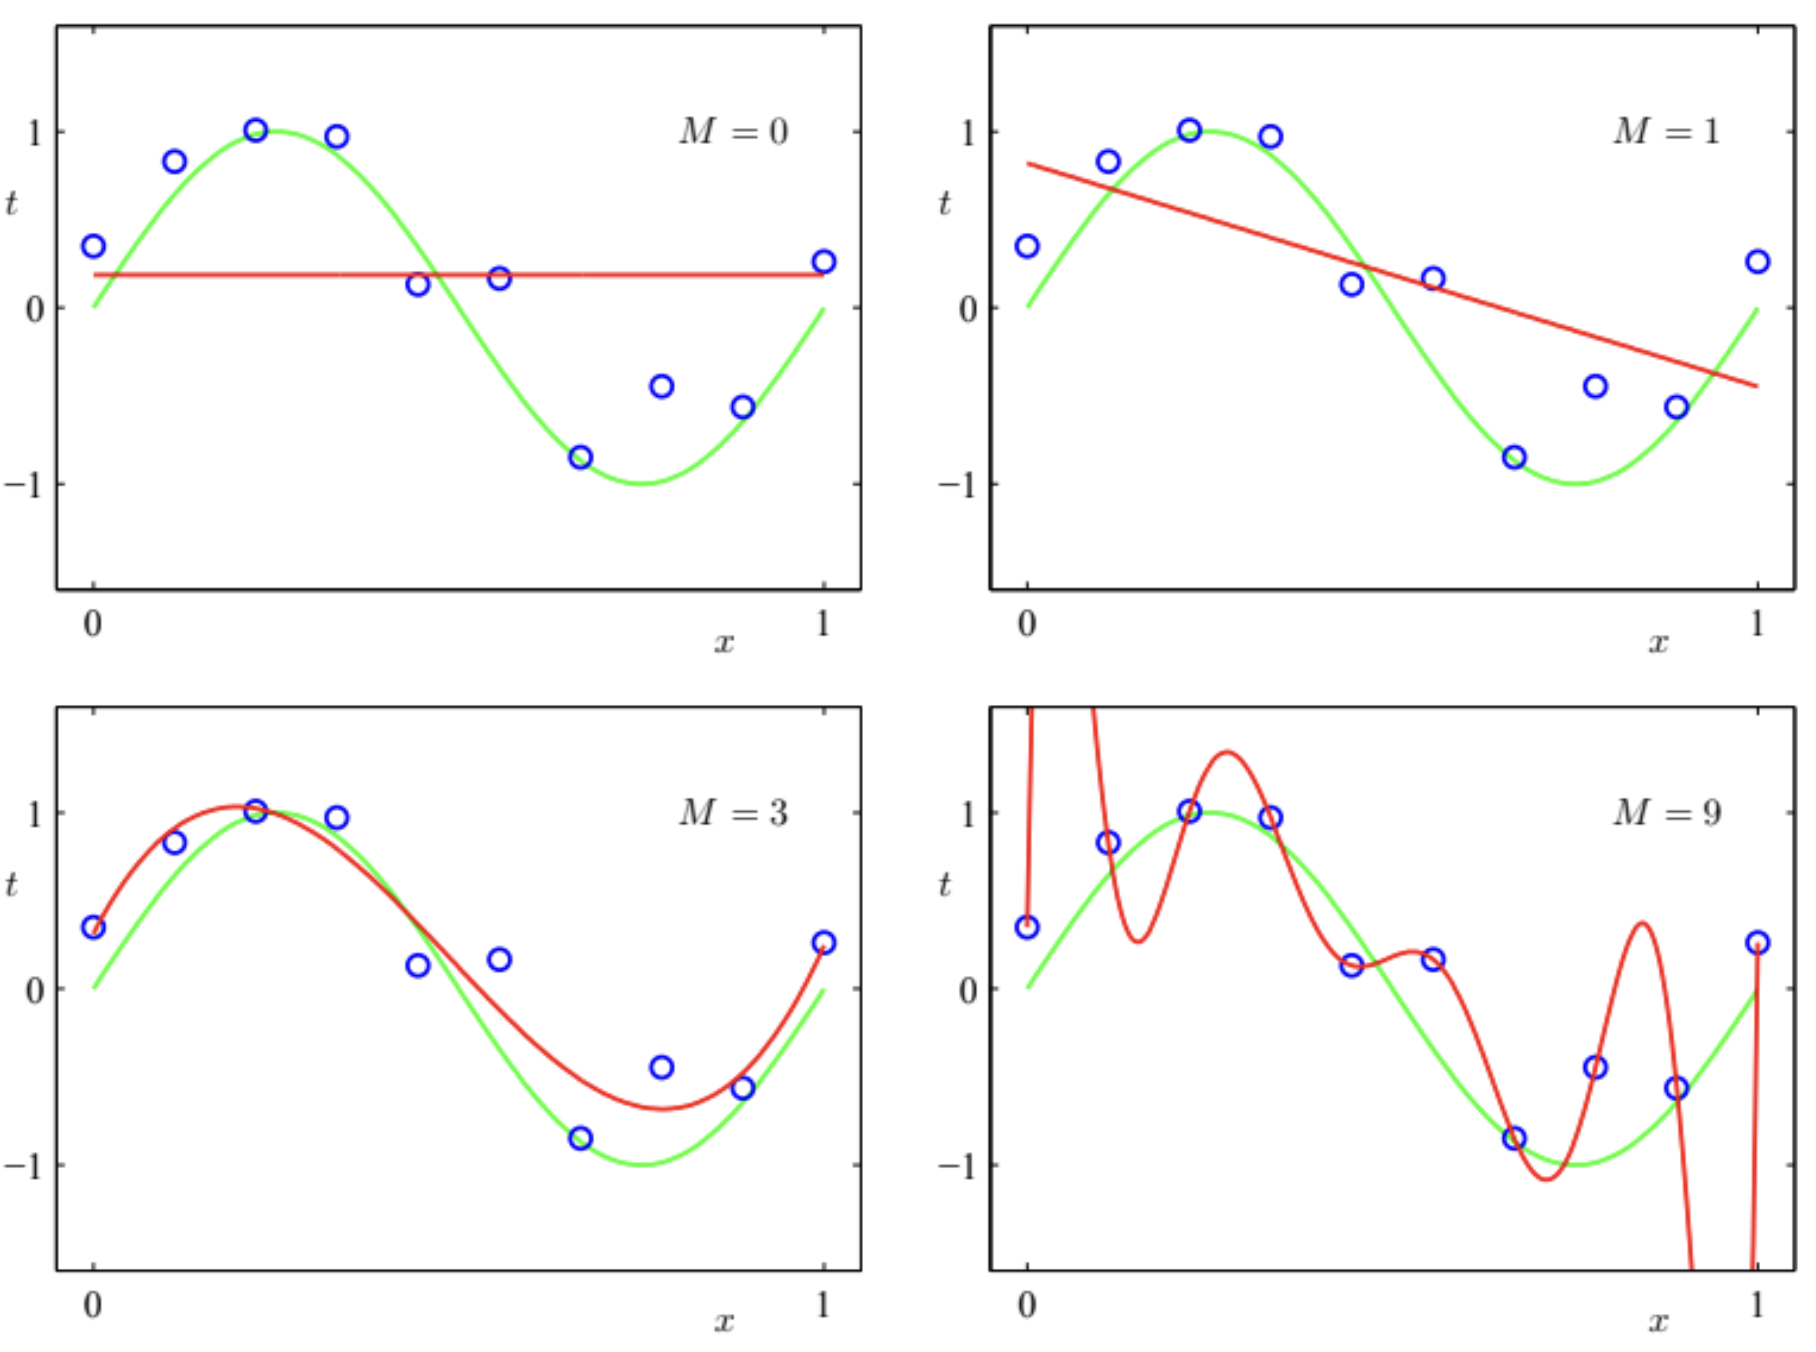
\includegraphics[width=0.5\textwidth]{images/lin_reg2.png}
\end{center} 
Let's now consider a noisy dataset\begin{align}
    &D=\{(\mathbf x_n,t_n)_{n=1}^N\}\\ 
    &f \text{ is the real target function }\\ 
    &t_n=f(\mathbf x_n)+\epsilon\\ 
    &\epsilon\in \R, \ \ \epsilon\sim 0
\end{align}
We assume that the noise on the samples have a Gaussian distribution\begin{equation}
    \Prob(\epsilon \text{ noise on sample }t_n)=\mathcal N(\epsilon,0,\beta^{-1})
\end{equation}
where $\beta^{-1}$ is the variance, we call $\beta$ the \textit{information coefficient}. Given such assumption:\begin{equation}
    \Prob(t_n|\mathbf x_n,\beta)=\mathcal N(t_n,f(\mathbf x_n),\beta^{-1})=\text{ probability that }t_n\text{ is the real value of }f(\mathbf x_n)
\end{equation}
Given a trained model $y$ with parameters $\mathbf w$, under this assumption we have\begin{equation}
    \Prob(t|\mathbf x,\mathbf w,\beta) 
\end{equation}
the probability that $t$ is the real outcome of $f(\mathbf x)$ given the model $\mathbf w$ and the information coefficient $\beta$, assuming that the samples are independent from each other, we have the maximum likelihood function:\begin{equation}
     \Prob(\{t_1\dots t_N\}|\{\mathbf x_1\dots\mathbf x_N\},\mathbf w,\beta) = 
     \prod_{n=1}^{N} \Prob(t_n|\mathbf x_n,\mathbf w,\beta) 
\end{equation}
given the assumptions:\begin{equation}
    \Prob(t_n|\mathbf x_n,\mathbf w,\beta) =\mathcal{N}(t_n|\mathbf w^T,\boldsymbol{\phi}(\mathbf x_n),\beta^{-1})
\end{equation}
we consider the log likelihood function:$$
 \ln \Prob(\{t_1\dots t_N\}|\{\mathbf x_1\dots\mathbf x_N\},\mathbf w,\beta) = 
     \sum_{n=1}^{N} \ln\Prob(t_n|\mathbf x_n,\mathbf w,\beta) $$
    Without entering in the details of the proof, it is shown that the log likelihood is proportional to the least squared error:\begin{equation}
        \ln \Prob(\{t_1\dots t_N\}|\{\mathbf x_1\dots\mathbf x_N\},\mathbf w,\beta)\simeq 
        \frac{1}{2}\sum_{n=1}^N(t_n-\mathbf w^T\boldsymbol{\phi}(\mathbf x_n))^2
    \end{equation}
    We can solve analytically the following problem:\begin{equation}
        \mathbf w^*=\arg\min_{\mathbf w}\frac{1}{2}\sum_{n=1}^N(t_n-\mathbf w^T\boldsymbol{\phi}(\mathbf x_n))^2
    \end{equation}
    If we consider the vector of labels $\mathbf t$ and the matrix\begin{equation}
        \Phi=\begin{pmatrix}
           \phi_0(\mathbf x_1)& \phi_1(\mathbf x_1)&\dots& \phi_M(\mathbf x_1)\\ 
            \phi_0(\mathbf x_1)&\phi_1(\mathbf x_2)&\dots& \phi_M(\mathbf x_2)\\
            \vdots &\ddots&\vdots
            \\ 
           \phi_0(\mathbf x_1)& \phi_1(\mathbf x_N)&\dots& \phi_M(\mathbf x_N)
        \end{pmatrix}=\begin{pmatrix}
            \boldsymbol{\phi}(\mathbf x_1)^T\\ 
             \boldsymbol{\phi}(\mathbf x_2)^T\\
             \vdots \\ 
              \boldsymbol{\phi}(\mathbf x_N)^T
        \end{pmatrix}
    \end{equation}
the least squared error can be rewritten in matrix form:\begin{equation}
    \frac{1}{2}\sum_{n=1}^N(t_n-\mathbf w^T\boldsymbol{\phi}(\mathbf x_n))^2=\frac{1}{2}(\mathbf t-\Phi\mathbf w)^T(\mathbf t-\Phi\mathbf w)
\end{equation}
the optimal value for $\mathbf w$ is\begin{equation}
    \mathbf w_{ML}=(\Phi^T\Phi)^{-1}\Phi^T\mathbf t=\Phi^{\dag}\mathbf t
\end{equation}
computing $\Phi^{\dag}\mathbf t$ is computationally expensive, we may consider a sequential algorithm, like the stochastic gradient descent.
$$\hat{\mathbf w}\leftarrow \hat{\mathbf w}-\eta\nabla E_S$$
with $\eta$ a learning parameter, $S\subset D$ and $E_S$ the least squared error evaluated on the samples in $S$.
\subsection{Regularization}
\redText{TODO}
\end{document}











